
%%
%% forked from https://gits-15.sys.kth.se/giampi/kthlatex kthlatex-0.2rc4 on 2020-02-13
%% expanded upon by Gerald Q. Maguire Jr.
%% This template has been adapted by Anders Sjögren to the University
%% Engineering Program in Computer Science at KTH ICT. Adaptation is the
%% translation of English headings into Swedish as the addition of Swedish
%% text. Original body text is deliberately left in English.

%% Conventions for todo notes:
% \todo[inline]{Comments/directions/... in English}
% \todo[inline, backgroundcolor=kth-lightblue]{Text på svenska}
% \todo[inline, backgroundcolor=kth-lightgreen]{English descriptions about formatting}

%% The template is designed to handle a thesis in English or Swedish
% set the default language to english or swedish by passing an option to the documentclass - this handles the inside tile page
% To optimize for digital output (this changes the color palette add the option: digitaloutput
% To use bibtex or biblatex - include one of these as an option
\documentclass[english, bibtex]{templates/kth/kththesis}
%\documentclass[swedish, biblatex]{kththesis}

% \usepackage[style=numeric,sorting=none,backend=biber]{biblatex}
\ifbiblatex
    %\usepackage[language=english,bibstyle=authoryear,citestyle=authoryear, maxbibnames=99]{biblatex}
     \usepackage[bibstyle=authoryear,citestyle=authoryear, maxbibnames=99,language=english]{biblatex}
    \addbibresource{references.bib}
    %\DeclareLanguageMapping{norsk}{norwegian}
\else
    % The line(s) below are for BibTeX
    \bibliographystyle{bibstyle/myIEEEtran}
    %\bibliographystyle{apalike}
\fi


% include a variety of packages that are useful
%%%%%%%%%%%%%%%%%%%%%%%%%%%%%% Packages %%%%%%%%%%%%%%%%%%%%%%%%%%%%%%
% The following is for use with the KTH cover when not using XeLaTeX or LuaLaTeX
%\ifxeorlua\relax
%\else
\usepackage[scaled]{helvet}
%\fi

%% The following are needed for generating the DiVA page(s)
\usepackage[force-eol=true]{scontents}              %% Needed to save lang, abstract, and keywords
\usepackage{pgffor}                 %% includes the foreach loop

%% Basic packages

%% Links
\usepackage{url}                %% Support for breaking URLs

%% Colorize
%\usepackage{color}
\PassOptionsToPackage{dvipsnames, svgnames}{xcolor}
\usepackage{xcolor}

\usepackage[normalem]{ulem}
\usepackage{soul}
\usepackage{xspace}
\usepackage{braket}

% to support units and decimal aligned columns in tables
\usepackage[locale=US]{siunitx}

\usepackage{balance}
\usepackage{stmaryrd}
\usepackage{booktabs}
\usepackage{graphicx}	        %% Support for images
\usepackage{multirow}	        %% Support for multirow columns in tables
\usepackage{tabularx}		    %% For simple table stretching
\usepackage{mathtools}
\usepackage{algorithm} 
\usepackage{algorithmic}  
\usepackage{amsmath}
\usepackage[linesnumbered,ruled,vlined,algo2e]{algorithm2e}
% can't use both algpseudocode and algorithmic packages
%\usepackage[noend]{algpseudocode}
%\usepackage{subfig}  %% cannot use both subcaption and subfig packages
\usepackage{optidef}
\usepackage{float}		        %% Support for more flexible floating box positioning
\usepackage{pifont}

%% some additional useful packages
% to enable rotated figures
\usepackage{rotating}	    	%% For text rotating
\usepackage{array}		        %% For table wrapping
\usepackage{mdwlist}            %% various list-related commands
\usepackage{setspace}           %% For fine-grained control over line spacing


\usepackage{enumitem}           %% to allow changes to the margins of descriptions


%% If you are going to include source code (or code snippets)
\usepackage{listings}		    %% For source code listing
%%\usepackage[cache=false]{minted} %% For source code highlighting
%%\usemintedstyle{borland}

\usepackage{bytefield}          %% For packet drawings


\setlength {\marginparwidth }{2cm} %leave some extra space for todo notes
\usepackage{todonotes}
\usepackage{notoccite} % do not number captions based on their appearance in the TOC


% Footnotes
\usepackage{perpage}
\usepackage[perpage,para,symbol]{footmisc} %% use symbols to ``number'' footnotes and reset which symbol is used first on each page


%% Various useful packages
%%----------------------------------------------------------------------------
%%   pcap2tex stuff
%%----------------------------------------------------------------------------
\usepackage{tikz}
\usepackage{colortbl}
\usetikzlibrary{arrows,decorations.pathmorphing,backgrounds,fit,positioning,calc,shapes}
\usepackage{pgfmath}	% --math engine
\newcommand\bmmax{2}
\usepackage{bm} % bold math


%% Managing titles
% \usepackage[outermarks]{titlesec}
%%%%%%%%%%%%%%%%%%%%%%%%%%%%%%%%%%%%%%%%%%%%%%%%%%%%%%%%%%%%%%%%%%%%%%
%\captionsetup[subfloat]{listofformat=parens}

% to include PDF pages
%\usepackage{pdfpages}


\usepackage{csquotes}               %% Recommended by biblatex
% to provide a float barrier use:
\usepackage{placeins}

\usepackage{comment}  %% Provides a comment environment
\usepackage{refcount}   %% to be able to get an expandable \getpagerefnumber

% for experiments with new cover
\usepackage{eso-pic}
\usepackage[absolute,overlay]{textpos}

% when the package is used, it draws boxes on the page showing the text, footnote, header, and margin regions of the page
%\usepackage{showframe}  
%\usepackage{printlen} % defines the printlength command to print out values of latex variable


%%% Local Variables:
%%% mode: latex
%%% TeX-master: t
%%% End:
% KTH colors for LaTeX documents
%
% Started from kthcolors by:
% Riccardo Sven Risuleo
% 2016-09-06 11:05:40
%
% from https://github.com/KTH-AC/kthcolors
%
% Adapted using the colors from "Graphic Profile Manual KTH" version 180604
% (i.e.. 2018-06-04) 
% see https://intra.kth.se/en/administration/kommunikation/grafiskprofil/kth-s-grafiska-profil-1.844676
% 
% G. Q. Maguire Jr.
% 2021-07-05
%

%\NeedsTexFormat{LaTeX2e}[1994/06/01]
%\ProvidesPackage{kthcolors}[2021/07/85 v3 Latex package with official KTH colors]

\RequirePackage{xcolor}
%% Primary colors
%% As of the new manual, there is only 1 primary color; but with three 
\definecolor{kth-blue}{RGB/cmyk}{25,84,166/0.849,0.494,0,0.349}
\colorlet{kth-blue80}{kth-blue!80!}
\colorlet{kth-blue40}{kth-blue!40!}

% these are no longer used as of 2018-06-04
%\definecolor{kth-red}{RGB/cmyk}{157,16,45/0,0.898,0.713,0.384}
%\definecolor{kth-green}{RGB/cmyk}{98,146,46/0.329,0,0.685,0.427}

%% Secondary colors
\definecolor{kth-lightblue}{RGB/cmyk}{36,160,216/0.833,0.259,0,0.153}
\colorlet{kth-lightblue80}{kth-lightblue!80!}
\colorlet{kth-lightblue40}{kth-lightblue!40!}

%\definecolor{kth-lightred}{RGB/cmyk}{228,54,62/0,0.763,0.728,0.106}
\definecolor{kth-lightred}{RGB}{216,84,151}
\colorlet{kth-lightred80}{kth-lightred!80!}
\colorlet{kth-lightred40}{kth-lightred!40!}

\definecolor{kth-lightgreen}{RGB/cmyk}{176,201,43/0.124,0,0.786,0.212} % olive
\colorlet{kth-lightgreen80}{kth-lightgreen!80!}
\colorlet{kth-lightgreen40}{kth-lightgreen!40!}

% Cool Gray 9C
%\definecolor{kth-coolgray}{RGB}{101,101,108}

% Cool Gray 10 suggested by Martin Krzywinski (see http://mkweb.bcgsc.ca/colorblind) 
\definecolor{kth-coolgray}{RGB}{99,102,106}
\colorlet{kth-coolgray80}{kth-coolgray!80!}
\colorlet{kth-coolgray40}{kth-coolgray!40!}

% Tertiary colors (yet more colors)
% All of these are no longer used
%\definecolor{kth-pink}{RGB/cmyk}{216,84,151/10,0.611,0.301,0.153}
%\definecolor{kth-yellow}{RGB/cmyk}{250,185,25/0,0.26,0.9,0.0196}
%\definecolor{kth-darkgray}{RGB/cmyk}{101,101,108/0.0648,0.0648,0,0.576}
%\definecolor{kth-middlegray}{RGB/cmyk}{189,188,188/0,0.00529,0.00529,0.259}
%\definecolor{kth-lightgray}{RGB/cmyk}{227,229,227/0.00873,0,0.00873,0.102}

%\DeclareOption{gray}{\colorlet{gray}{kth-darkgray}}

% These versions are designed to meet accessability requirements for digital media
% Note that the palette is more limited than for the print version of the colors
\ifdigitaloutput
    % primary color
    \definecolor{kth-blue}{HTML}{1954A6} % Deep sea
    \definecolor{kth-blue80}{HTML}{5E87C0}

    % Secondary colors
    \definecolor{kth-lightblue}{HTML}{2191C4} % Stratosphere
    \definecolor{kth-lightred}{HTML}{D02F80} % Fluorescence
    \definecolor{kth-lightred80}{HTML}{D95599}
    \definecolor{kth-lightgreen}{HTML}{62922E} % Front-lawn
    \definecolor{kth-coolgray}{HTML}{65656C} % Office
    \definecolor{kth-coolgray80}{HTML}{848489}
\fi



%\glsdisablehyper
%\makeglossaries 
%\makenoidxglossaries
%%%% Local Variables:
%%% mode: latex
%%% TeX-master: t
%%% End:

% The form of the entries in this file is \newacronym{label}{acronym}{phrase}
%                                      or \newacronym[options]{label}{acronym}{phrase}
% see "User Manual for glossaries.sty" for the  details about the options, one example is shown below
% note the specification of the long form plural in the line below
\newacronym[longplural={Debugging Information Entities}]{DIE}{DIE}{Debugging Information Entity}
%
% The following example also uses options
\newacronym[plural={OSes}, firstplural={operating systems (OSes)}]{OS}{OS}{operating system}

% note the use of a non-breaking dash in long text for the following acronym
\newacronym{IQL}{IQL}{Independent Q‑Learning}

\newacronym{LAN}{LAN}{Local Area Network}
% note the use of a non-breaking dash in the following acronym
\newacronym{WiFi}{Wi-Fi}{Wireless Fidelity}

\newacronym{WLAN}{WLAN}{Wireless Local Area Network}
\newacronym{UN}{UN}{United Nations}
\newacronym{SDG}{SDG}{Sustainable Development Goal}
                %load the acronyms file

\makeatletter
\newcommand{\DeclareLatinAbbrev}[2]{%
  \DeclareRobustCommand{#1}{%
    \@ifnextchar{.}{\textit{#2}}{%
      \@ifnextchar{,}{\textit{#2.}}{%
        \@ifnextchar{!}{\textit{#2.}}{%
          \@ifnextchar{?}{\textit{#2.}}{%
            \@ifnextchar{)}{\textit{#2.}}{%
              {\textit{#2.,\ }}}}}}}}%
}
\makeatother
\DeclareLatinAbbrev{\eg}{e.g}
\DeclareLatinAbbrev{\Eg}{E.g}
\DeclareLatinAbbrev{\ie}{i.e}
\DeclareLatinAbbrev{\Ie}{I.e}
\DeclareLatinAbbrev{\etc}{etc}
\DeclareLatinAbbrev{\etal}{et~al}

\def\first {$(i)$\xspace}
\def\Second{$(ii)$\xspace}
\def\third {$(iii)$\xspace}
\def\fourth{$(iv)$\xspace}
\def\fifth {$(v)$\xspace}
\def\sixth {$(vi)$\xspace}
\def\seventh{$(vii)$\xspace}
\def\eighth{$(viii)$\xspace}

%%% custom definitions
%% Coloring the links!
\newcommand\myshade{75} % Usage: red!\myshade!black

\definecolor{ForestGreen} {RGB}{34,  139,  34}
\definecolor{HeraldRed2}   {rgb}{0.81, 0.12, 0.15}

\newcommand{\refscolor} {blue}
\newcommand{\linkscolor}{HeraldRed2}
\newcommand{\urlscolor} {ForestGreen}

%% Some definitions of used colors
%\definecolor{darkblue}{rgb}{0.0,0.0,0.3} %% define a color called darkblue
%\definecolor{darkred}{rgb}{0.4,0.0,0.0}
%\definecolor{red}{rgb}{0.7,0.0,0.0}
%\definecolor{lightgrey}{rgb}{0.8,0.8,0.8} 
%\definecolor{grey}{rgb}{0.6,0.6,0.6}
%\definecolor{darkgrey}{rgb}{0.4,0.4,0.4}
%\definecolor{aqua}{rgb}{0.0, 1.0, 1.0}

% For runin headings
\newcommand{\smartparagraph}[1]{\vspace{.05in}\noindent\textbf{#1}}

%% Table of Contents (ToC) depth 
\setcounter{secnumdepth}{4} % how many sectioning levels to assign numbers to
\setcounter{tocdepth}{4}    % how many sectioning levels to show in ToC

%% Limit hyphenation
\hyphenpenalty=9000
\tolerance=5000
% Reduce hyphenation as much as possible:
%\hyphenpenalty=15000
%\tolerance=1000

% Use grouping for numbers that are 4 or more digits long
\sisetup{group-minimum-digits=4}
  % load some additional definitions to make writing more consistent

% The following is needed in conjunction with generating the DiVA data with abstracts and keywords using the scontents package and a modified listings environment
%\usepackage{listings}   %  already included
\ExplSyntaxOn
\newcommand\typestoredx[2]{\expandafter\__scontents_typestored_internal:nn\expandafter{#1} {#2}}
\ExplSyntaxOff
\makeatletter
\let\verbatimsc\@undefined
\let\endverbatimsc\@undefined
\lst@AddToHook{Init}{\hyphenpenalty=50\relax}
\makeatother


\lstnewenvironment{verbatimsc}
    {
    \lstset{%
        basicstyle=\ttfamily\tiny,
        backgroundcolor=\color{white},
        %basicstyle=\tiny,
        %columns=fullflexible,
        columns=[l]fixed,
        language=[LaTeX]TeX,
        %numbers=left,
        %numberstyle=\tiny\color{gray},
        keywordstyle=\color{red},
        breaklines=true,                 % sets automatic line breaking
        breakatwhitespace=true,          % sets if automatic breaks should only happen at whitespace
        %keepspaces=false,
        breakindent=0em,
        %fancyvrb=true,
        frame=none,                     % turn off any box
        postbreak={}                    % turn off any hook arrow for continuation lines
    }
}{}


%% definition of new command for bytefield package
% \newcommand{\colorbitbox}[3]{%
% 	\rlap{\bitbox{#2}{\color{#1}\rule{\width}{\height}}}%
% 	\bitbox{#2}{#3}}

%% Acronyms
% note that nonumberlist - removes the cross references to the pages where the acronym appears
% note that nomain - does not produce a main glossary, this only acronyms will be in the glossary
% note that nopostdot - will present there being a period at the end of each entry
\usepackage[acronym, section=section, nonumberlist, nomain, nopostdot]{glossaries}
\usepackage[automake]{glossaries-extra}
\ifinswedish
    %\usepackage{glossaries-swedish}
\fi

% Because backref is not compatible with biblatex
\ifbiblatex
    \usepackage[plainpages=false]{hyperref}
\else
    \usepackage[
    backref=page,
    pagebackref=false,
    plainpages=false,
                            % PDF related options
    unicode=true,           % Unicode encoded PDF strings
    bookmarks=true,         % generate bookmarks in PDF files
    bookmarksopen=false,    % Do not automatically open the bookmarks in the PDF reading program
    pdfpagemode=UseNone,    % None, UseOutlines, UseThumbs, or FullScreen
    ]{hyperref}
    \usepackage{backref}
    %
    % Customize list of backreferences.
    % From https://tex.stackexchange.com/a/183735/1340
    \renewcommand*{\backref}[1]{}
    \renewcommand*{\backrefalt}[4]{%
    \ifcase #1%
          \or [Page~#2.]%
          \else [Pages~#2.]%
    \fi%
    }
\fi
\usepackage[all]{hypcap}	%% prevents an issue related to hyperref and caption linking


% packages that have to be included after hyperref
\usepackage{doi}
\usepackage{cleveref}           %% Replace Section with a symbol


%\glsdisablehyper
\makeglossaries
%%% Local Variables:
%%% mode: latex
%%% TeX-master: t
%%% End:

% The form of the entries in this file is \newacronym{label}{acronym}{phrase}
%                                      or \newacronym[options]{label}{acronym}{phrase}
% see "User Manual for glossaries.sty" for the  details about the options, one example is shown below
% note the specification of the long form plural in the line below
\newacronym[longplural={Debugging Information Entities}]{DIE}{DIE}{Debugging Information Entity}
%
% The following example also uses options
\newacronym[plural={OSes}, firstplural={operating systems (OSes)}]{OS}{OS}{operating system}

% note the use of a non-breaking dash in long text for the following acronym
\newacronym{IQL}{IQL}{Independent Q‑Learning}

\newacronym{LAN}{LAN}{Local Area Network}
% note the use of a non-breaking dash in the following acronym
\newacronym{WiFi}{Wi-Fi}{Wireless Fidelity}

\newacronym{WLAN}{WLAN}{Wireless Local Area Network}
\newacronym{UN}{UN}{United Nations}
\newacronym{SDG}{SDG}{Sustainable Development Goal}
                %load the acronyms file

% insert the configuration information with author(s), examiner, supervisor(s), ...
%% Information for inside title page
\authorsLastname{Olsson}
\authorsFirstname{Glenn}
\email{glennol@kth.se}
\kthid{u18orpa8}
\authorsSchool{\schoolAcronym{EECS}}

%second author information

%External cooperation information
\hostcompany{Cal Poly}
%\hostorganization{CERN}   \% if there was a host organization

%Supervisor(s) information
\supervisorAsLastname{Ghasemirahni}
\supervisorAsFirstname{Hamid}
\supervisorAsEmail{hamidgr@kth.se}
\supervisorAsKTHID{u1fz5jtv}
\supervisorAsSchool{\schoolAcronym{None}}
\supervisorAsDepartment{Computer Science}
\supervisorBsLastname{Peterson}
\supervisorBsFirstname{Zachory}
\supervisorBsEmail{znjpeterson@gmail.com}
\supervisorBsOrganization{Cal Poly}

%Examiner information
\examinersLastname{Maguire Jr}
\examinersFirstname{Gerald Quentin}
\examinersEmail{maguire@kth.se}
\examinersKTHID{u1d13i2c}
\examinersSchool{\schoolAcronym{None}}
\examinersDepartment{Computer Science}

%Date

\date{\today}

%course and program information
\courseCycle{2}
\courseCode{DA231X}
\edprogram{Master's Programme, Computer Science, 120 credits}
\programcode{TCSCM}
\degreeName{Degree of Master (120 credits)}
%%%%% for DiVA's National Subject Category information
%%% Enter one or more 3 or 5 digit codes
%%% See https://www.scb.se/contentassets/3a12f556522d4bdc887c4838a37c7ec7/standard-for-svensk-indelning--av-forskningsamnen-2011-uppdaterad-aug-2016.pdf
%%% See https://www.scb.se/contentassets/10054f2ef27c437884e8cde0d38b9cc4/oversattningsnyckel-forskningsamnen.pdf
%%%%
%%%% Some examples of these codes are shown below:
% 102 Data- och informationsvetenskap (Datateknik)    Computer and Information Sciences
% 10201 Datavetenskap (datalogi) Computer Sciences
% 10202 Systemvetenskap, informationssystem och informatik (samhällsvetenskaplig inriktning under 50804)
% Information Systems (Social aspects to be 50804)
% 10203 Bioinformatik (beräkningsbiologi) (tillämpningar under 10610)
% Bioinformatics (Computational Biology) (applications to be 10610)
% 10204 Människa-datorinteraktion (interaktionsdesign) (Samhällsvetenskapliga aspekter under 50803) Human Computer Interaction (Social aspects to be 50803)
% 10205 Programvaruteknik Software Engineering
% 10206 Datorteknik Computer Engineering
% 10207 Datorseende och robotik (autonoma system) Computer Vision and Robotics (Autonomous Systems)
% 10208 Språkteknologi (språkvetenskaplig databehandling) Language Technology (Computational Linguistics)
% 10209 Medieteknik Media and Communication Technology
% 10299 Annan data- och informationsvetenskap Other Computer and Information Science
%%%
% 202 Elektroteknik och elektronik Electrical Engineering, Electronic Engineering, Information Engineering
% 20201 Robotteknik och automation Robotics
% 20202 Reglerteknik Control Engineering
% 20203 Kommunikationssystem Communication Systems
% 20204 Telekommunikation Telecommunications
% 20205 Signalbehandling Signal Processing
% 20206 Datorsystem Computer Systems
% 20207 Inbäddad systemteknik Embedded Systems
% 20299 Annan elektroteknik och elektronik Other Electrical Engineering, Electronic Engineering, Information Engineering
%% Example for a thesis in Computer Science and Computer Systems

%National Subject Categories information
\nationalsubjectcategories{10201}

% Added by Glenn
\subjectArea{Computer Science and Engineering}
\courseCredits{120}

\title{This is the title in the language of the thesis}
\subtitle{An subtitle in the language of the thesis}

% give the alternative title - i.e., if the thesis is in English, then give a Swedish title
\alttitle{Detta är den svenska översättningen av titeln}
\altsubtitle{Detta är den svenska översättningen av undertiteln}
% alternative, if the thesis is in Swedish, then give an English title
%\alttitle{This is the English translation of the title}
%\altsubtitle{This is the English translation of the subtitle}

% Enter the English and Swedish keywords here for use in the PDF meta data _and_ for later use
% following the respective abstract.
% Try to put the words in the same order in both languages to facilitate matching. For example:
\EnglishKeywords{Canvas Learning Management System, Docker containers, Performance tuning}
\SwedishKeywords{Canvas Lärplattform, Dockerbehållare, Prestandajustering}

%%%%% For the oral presentation
%% Add this information once your examiner has scheduled your oral presentation
\presentationDateAndTimeISO{2022-03-15 13:00}
\presentationLanguage{eng}
\presentationRoom{via Zoom https://kth-se.zoom.us/j/ddddddddddd}
\presentationAddress{Isafjordsgatan 22 (Kistagången 16)}
\presentationCity{Stockholm}

% When there are multiple opponents, separate their names with '\&'
% Opponent's information
\opponentsNames{A. B. Normal \& A. X. E. Normalè}

% Once a thesis is approved by the examiner, add the TRITA number
% for entering the TRITA number for a thesis
\trita{TRITA-EECS-EX}{2022:00}

% Put the title, author, and keyword information into the PDF meta information
% This file contains the LaTeX to add information to the PDF file (specifically, author(s), title(s), and keywords
% It uses the hyperref package and should be be included before the \begin{document}
%
% I want to acknowledge the inspiration of Karl Voit's template for TU Graz that inspired me to add the PDF document information
% For more information about his template see https://github.com/novoid/LaTeX-KOMA-template
% Note that this template does not use anything from his template other than the names of the information for the PDF meta fields, i.e., mytitle, myauthor, and mykeywords together with the idea of defining the corresponding newcommand to set the relevant hyperref parameters.

\makeatletter
\ifx\@subtitle\@empty
    \newcommand{\mytitle}{\@title}
\else
    \newcommand{\mytitle}{\@title: \@subtitle}
\fi
\makeatother

\hypersetup{
     pdftitle={\mytitle}        % Title field
}

\makeatletter
\ifx\@secondAuthorsLastname\@empty
    \newcommand{\myauthor}{\@authorsFirstname\space\@authorsLastname} 
\else
    \ifinswedish
    \newcommand{\myauthor}{\@authorsFirstname\space\@authorsLastname\space\relax och\space\@secondAuthorsFirstname \@secondAuthorsLastname}
    \else
        \newcommand{\myauthor}{\@authorsFirstname\space\@authorsLastname\space\relax and\space\@secondAuthorsFirstname \@secondAuthorsLastname}
    \fi
\fi
\makeatother

\hypersetup{
     pdfauthor={\myauthor}      % Author field
}

% Put the alternative title (and subtitle) into the PDF Subject meta
\makeatletter
\ifx\@altsubtitle\@empty\relax
    \newcommand{\myalttitle}{\@alttitle}
\else
    \newcommand{\myalttitle}{\@alttitle: \@altsubtitle}
\fi
\makeatother

\hypersetup{
     pdfsubject={\myalttitle}        % Subject field
}

\makeatletter
\ifx\@EnglishKeywords\@empty
    \ifx\@SwedishKeywords\@empty
        \newcommand{\mykeywords}{}
    \else
    \newcommand{\mykeywords}{\@SwedishKeywords}
    \fi
\else
    \ifx\@SwedishKeywords\@empty
        \newcommand{\mykeywords}{\@EnglishKeywords}
    \else
        \ifinswedish
            \newcommand{\mykeywords}{\@SwedishKeywords, \@EnglishKeywords}
        \else
            \newcommand{\mykeywords}{\@EnglishKeywords, \@SwedishKeywords}
        \fi
    \fi
\fi
\makeatother

\hypersetup{
     pdfkeywords={\mykeywords}        % Keywords field
}        
% I have _not_ set the following fields:
%    pdfcreator             % Creator field
%    pdfproducer            % Producer field
 


% the custom colors and the commands are defined in defines.tex    
\hypersetup{
	colorlinks  = true,
	breaklinks  = true,
	linkcolor   = \linkscolor,
	urlcolor    = \urlscolor,
	citecolor   = \refscolor,
	anchorcolor = black
}


\begin{document}
%\selectlanguage{swedish}
%
\selectlanguage{english}

%%% Set the numbering for the title page to a numbering series not in the preface or body
\pagenumbering{alph}
\kthcover
\titlepage
% document/book information page
\bookinfopage

% Frontmatter includes the abstracts and table-of-contents
\frontmatter
\setcounter{page}{1}
\begin{abstract}
% The first abstract should be in the language of the thesis.
% Abstract fungerar på svenska också.
  \markboth{\abstractname}{}
\begin{scontents}[store-env=lang]
eng
\end{scontents}
%%% The contents of the abstract (between the begin and end of scontents) will be saved in LaTeX format
%%% and output on the page(s) at the end of the thesis with information for DiVA facilitating the correct
%%% entry of the meta data for your thesis.
%%% These page(s) will be removed before the thesis is inserted into DiVA.
\begin{scontents}[store-env=abstracts,print-env=true]

% \todo[inline, backgroundcolor=kth-lightgreen]{All theses at KTH are \textbf{required} to have an abstract in both \textit{English} and \textit{Swedish}.}

% \todo[inline, backgroundcolor=kth-lightgreen]{GLENNE HARRIE OLLESSON Exchange students many want to include one or more abstracts in the language(s) used in their home institutions to avoid the need to write another thesis when returning to their home institution.}

% \todo[inline]{Keep in mind that most of your potential readers are only going to read your \texttt{title} and \texttt{abstract}. This is why it is important that the abstract give them enough information that they can decide is this document relevant to them or not. Otherwise the likely default choice is to ignore the rest of your document.\\

% A abstract should stand on its own, i.e., no citations, cross references to the body of the document, acronyms must be spelled out, \ldots .\\

% Write this early and revise as necessary. This will help keep you focused on what you are trying to do.}

Many \glspl{OWS} today, such as Flickr and Twitter, provide users with the possibility to post images that are stored on the platform for free. This thesis explores creating a cryptographically secure filesystem that stores its data on an online web service by encoding the encrypted data as images. Images have been selected as the target as more data can usually be stored in image posts than text posts on \glspl{OWS}. The proposed filesystem, named \gls{FFS}, provides users with free, deniable, and cryptographic storage by exploiting the storage provided by online web services. The thesis analyzes and compares the performance of \gls{FFS} against two other filesystems and a version of \gls{FFS} that does not use an \gls{OWS}. While \gls{FFS} has performance limitations that make it \mbox{non-viable} as a \mbox{general-purpose} filesystem, such as a substitute for the local filesystem on a computer; however, \gls{FFS} provides security benefits compared to other \mbox{cloud-based} filesystems specifically by providing \mbox{end-to-end} encryption, authenticated encryption, and plausible deniability of the data. Furthermore, being a \mbox{cloud-based} filesystem, \gls{FFS} can be mounted on any computer with the same operating system, given the correct secrets. 

% TODO: Add more about environmental etc.

\end{scontents}
% \todo[inline, backgroundcolor=kth-lightgreen]{The following are some notes about what can be included (in terms of LaTeX) in your abstract.}
% Choice of typeface with \textbackslash textit, \textbackslash textbf, and \textbackslash texttt:  \textit{x}, \textbf{x}, and \texttt{x}

% Text superscripts and subscripts with \textbackslash textsubscript and \textbackslash textsuperscript: A\textsubscript{x} and A\textsuperscript{x}

% Some useful symbols: \textbackslash textregistered, \textbackslash texttrademark, and \textbackslash textcopyright. For example, 
% copyright symbol: \textbackslash textcopyright Maguire 2022, and some superscripts: \textbackslash textsuperscript\{99m\}Tc, A\textbackslash textsuperscript\{*\}, A\textbackslash textsuperscript\{\textbackslash textregistered\}, and A\textbackslash texttrademark : \textcopyright Maguire 2022, and some superscripts: \textsuperscript{99m}Tc, A\textsuperscript{*}, A\textsuperscript{\textregistered}, and A\texttrademark. Another example: H\textbackslash textsubscript\{2\}O: H\textsubscript{2}O

% Simple environment with begin and end: itemize and enumerate and within these \textbackslash item

% The following macros can be used: \textbackslash eg, \textbackslash Eg, \textbackslash ie, \textbackslash Ie, \textbackslash etc, and \textbackslash etal: \eg, \Eg, \ie, \Ie, \etc, and \etal

% The following macros for numbering with lower case roman numerals: \textbackslash first, \textbackslash second, \textbackslash third, \textbackslash fourth, \textbackslash fifth, \textbackslash sixth, \textbackslash seventh, and \textbackslash eighth: \first, \second, \third, \fourth, \fifth, \sixth, \seventh, and \eighth.

% Equations using \textbackslash( xxxx \textbackslash) or \textbackslash[ xxxx \textbackslash] can be used in the abstract. For example: \( (C_5O_2H_8)_n \)
% or \[ \int_{a}^{b} x^2 \,dx \]


% Even LaTeX comments can be handled, for example: \% comment at end

\subsection*{Keywords}
\begin{scontents}[store-env=keywords,print-env=true]
% If you set the EnglishKeywords earlier, you can retrieve them with:
\InsertKeywords{english}
% If you did not set the EnglishKeywords earlier then simply enter the keywords here:
% comma separate keywords, such as: Canvas Learning Management System, Docker containers, Performance tuning
\end{scontents}

Choose the most specific keyword from those used in your domain, see for example: the ACM Computing Classification System ({\small \url{https://www.acm.org/publications/computing-classification-system/how-to-use})},
the IEEE Taxonomy ({\small \url{https://www.ieee.org/publications/services/thesaurus-thank-you.html}}), PhySH (Physics Subject Headings)\linebreak[4] ({\small \url{https://physh.aps.org/}}), \ldots or keyword selection tools such as the  National Library of Medicine's Medical Subject Headings (MeSH)  ({\small \url{https://www.nlm.nih.gov/mesh/authors.html}}) or Google's Keyword Tool ({\small \url{https://keywordtool.io/}})\\

\textbf{Mechanics}:
\begin{itemize}
  \item The first letter of a keyword should be set with a capital letter and proper names should be capitalized as usual.
  \item Spell out acronyms and abbreviations.
  \item Avoid "stop words" - as they generally carry little or no information.
  \item List your keywords separated by commas (",").
\end{itemize}    
Since you should have both English and Swedish keywords - you might think of ordering them in corresponding order (\ie, so that the n\textsuperscript{th} word in each list correspond) - this makes it easier to mechanically find matching keywords.
\end{abstract}
\cleardoublepage
\babelpolyLangStart{swedish}
\begin{abstract}
    \markboth{\abstractname}{}
\begin{scontents}[store-env=lang]
swe
\end{scontents}
\begin{scontents}[store-env=abstracts,print-env=true]

% \todo[inline, backgroundcolor=kth-lightblue]{Alla avhandlingar vid KTH \textbf{måste ha} ett abstrakt på både \textit{engelska} och \textit{svenska}.\\
% Om du skriver din avhandling på svenska ska detta göras först (och placera det som det första abstraktet) - och du bör revidera det vid behov.}

% \todo[inline]{If you are writing your thesis in English, you can leave this until the draft version that goes to your opponent for the written opposition. In this way you can provide the English and Swedish abstract/summary information that can be used in the announcement for your oral presentation.\\

% If you are writing your thesis in English, then this section can be a summary targeted at a more general reader. However, if you are writing your thesis in Swedish, then the reverse is true – your abstract should be for your target audience, while an English summary can be written targeted at a more general audience.\\

% This means that the English abstract and Swedish sammnfattning  
% or Swedish abstract and English summary need not be literal translations of each other.
% }
% \todo[inline, backgroundcolor=kth-lightred]{Do not use the \textbackslash glspl\{\} macro in an abstract that is not in English, as my programs do not know how to generate plurals in other languages. Instead you will need to spell these terms out or give the proper plural form.}

% \todo[inline, backgroundcolor=kth-lightgreen]{The abstract in the language used for the thesis should be the first abstract, while the Summary/Sammanfattning in the other language can follow}

Sammanfattning på svenska

\end{scontents}
\subsection*{Nyckelord}
\begin{scontents}[store-env=keywords,print-env=true]
% SwedishKeywords were set earlier, hence we can use alternative 2
\InsertKeywords{swedish}
\end{scontents}

\end{abstract}
\babelpolyLangStop{swedish}

\cleardoublepage

\section*{Acknowledgments }
\markboth{Acknowledgments}{}

\noindent
Thanks to:
\begin{itemize}
    \item I would like to thank xxxx for having yyyy.
\end{itemize}


\acknowlegmentssignature

\fancypagestyle{plain}{}
\renewcommand{\chaptermark}[1]{ \markboth{#1}{}} 
\tableofcontents
  \markboth{\contentsname}{}

\cleardoublepage
\listoffigures

\cleardoublepage

\listoftables
\cleardoublepage
\lstlistoflistings % \todo[inline, backgroundcolor=kth-lightgreen]{If you have listings in your thesis. If not, then remove this preface page.}
\cleardoublepage
% Align the text expansion of the glossary entries
\newglossarystyle{mylong}{%
  \setglossarystyle{long}%
  \renewenvironment{theglossary}%
     {\begin{longtable}[l]{@{}p{\dimexpr 2cm-\tabcolsep}p{0.8\hsize}}}% <-- change the value here
     {\end{longtable}}%
 }
%\glsaddall
%\printglossaries[type=\acronymtype, title={List of acronyms}]
\printglossary[style=mylong, type=\acronymtype, title={List of acronyms and abbreviations}]
%\printglossary[type=\acronymtype, title={List of acronyms and abbreviations}]

%% The following label is essential to know the page number of the last page of the preface
%% It is used to computer the data for the "For DIVA" pages
\label{pg:lastPageofPreface}
% Mainmatter is where the actual contents of the thesis goes
\mainmatter
\glsresetall
\renewcommand{\chaptermark}[1]{\markboth{#1}{}}
\selectlanguage{english}


\chapter{Introduction}
\label{ch:introduction}
% 	todo[inline, backgroundcolor=kth-lightblue]{svensk: Introduktion}


% \todo[inline, backgroundcolor=kth-lightblue]{Ofta kommer problemet och problemägaren
%   från industrin där man önskar en specifik lösning på ett specifikt
%   problem. Detta är ofta ”för smalt” definierat och ger ofta en ”för smal”
%   lösning för att resultatet skall vara intressant ur ett mer allmänt
%   ingenjörsperspektiv och med ”nya” erfarenheter som resultat. Fundera
%   tillsammans med projektets intressenter (student, problemägare och akademi)
%   hur man skulle kunna använda det aktuella problemet/förslaget för att
%   undersöka någon ingenjörsaspekt och vars resultat kan ge ny eller
%   kompletterande erfarenhet till ingenjörssamfundet och vetenskapen.\\
  
%   Examensarbetet handlar då om att ta fram denna nya ”erfarenhet” och på köpet
%   löser man en del eller hela delen av det ursprungliga problemet.\\

%   Erfarenheten kommer ur en frågeställning som man i examensarbetet försöker
%   besvara med tidigare och andras erfarenhet, egna eller modifierade metoder som
%   ger ett resultat vilket kan användas för att diskutera ett svar på
%   undersökningsfrågan.\\

%   Detta stycke skall alltså, förutom det ursprungliga ”smala” problemet,
%   innehålla  vad som skall undersökas för att skapa ny ingenjörserfarenhet
%   och/eller vetenskap.
% }

% \todo[inline, backgroundcolor=kth-lightgreen]{The first paragraph after a heading is not indented, all of the
%   subsequent paragraphs have their first line indented.}
  
% This chapter describes the specific problem that this thesis addresses, the context of the problem, the
% goals of this thesis project, and outlines the structure of the thesis.\\

% \todo[inline]{Give a general introduction to the area. (Remember to use appropriate references in this and all other sections.)}

% One can use either biblatex or bibtex - set as the option for the document at the top of this file
  % \ifbiblatex
% \todo[inline, backgroundcolor=kth-lightgreen]{We use the \emph{biblatex} package to handle our references.  We
% use the command \texttt{parencite} to get a reference in parenthesis, like
% this \textbackslash parencite\{heisenberg2015\} resulting in \parencite{heisenberg2015}.  It is also possible to include the author as part of the sentence using \texttt{textcite}, like talking about the work of \textbackslash textcite\{einstein2016\} resulting in \textcite{einstein2016}.\\
% This also means that you have to change the include files to include biblatex and change the way that the reference.bib file is included.}
  % \else
% \todo[inline, backgroundcolor=kth-lightgreen]{We use the \emph{bibtex} package to handle our references.  We therefore
% use the command \textbackslash cite\{farshin\_make\_2019\}. For example, Farshin, \etal described how to improve LLC

% at \SI{200}{Gbps}.}
  % \fi

% \todo[inline, backgroundcolor=kth-lightgreen]{Use the glossaries package to help yourself and your readers.
% Add the acronyms and abbreviations to templates/kth/lib/acronyms.tex. Some examples are shown below:}
% In this thesis we will examine the use of \glspl{LAN}. In this thesis we will
% assume that \glspl{LAN} include \glspl{WLAN}, such as \gls{WiFi}.

Year after year, people increase their total data storage used for obvious reasons. Cameras increase their resolution leading to images and videos taking even more space. With storage being cheap and easily usable, files do not need to be deleted thus the data accumulates. % FIXME: CITATION NEEDED?
This means that users will require more and more storage throughout their lifetime, and even potentially beyond their lifetime if their descendants want to keep these files. System storage in our hardware devices often increases with new product cycles. Today you can keep hundreds of gigabytes in your pocket at a reasonable cost. % FIXME: COMPARE iPHONE FROM LIKE 10 YEARS AGO AND TODAY - STORAGE AVAILIABLE, INCREASED. LOWEST TIER VS HIGHEST TIER
Along with increasing device storage and cloud storage, the aggregate storage capacity available to users is increasing. For instance, Apple's iCloud service allows users to store up to \SI{2}{\tera\byte} of data in the cloud for a few U.S. Dollars per month. % FIXME: CITE??
Even though the cost per month is not a lot, after many months this cost accumulates and you as a user become more and more dependent on this storage, especially as you do not want to spend time looking through all your data and remove some files to save space. % FIXME: FIND SOMETHING THAT USERS NEVER DOWNGRADES THEIR STORAGE - MUST EXIST
With increased pricing or increased space, the total cost will be even higher.

Social media platforms such as Twitter, Flickr, and Facebook have many millions of daily users that post texts and images (for example, of their cats or funny videos). According to Henna Kermani at Twitter, they processed ~\SI{200}{\giga\byte} of image data every second in 2016\,\cite{MobileScaleLondona}. The difference between the photos posted on Twitter compared to the ones stored on cloud services such as Google Drive is that the images on Twitter are stored for free for the user, for what seems to be an indefinite period. However, there is no obligation for these services to save it forever, they do reserve the right to remove any content at any time, as stated in their terms of service\footnote{\url{https://twitter.com/en/tos}}. There is also no specified maximum lifespan of these posts. While Google Drive and similar services often have a free-tier of storage, Twitter does not have a specified upper limit of how many images or tweets one can make, but such constraints can be imposed on specific users whenever Twitter wishes as is stated in their terms of service\footnote{\url{https://twitter.com/en/tos}}.

\section{Project Overview}

This project intends to create a filesystem called \textit{Fejk File System} (FFS) which takes advantage of online web services, such as Twitter, for the actual storage. The idea is to save the user's files by posting or sending an encrypted version of the file as posts or private messages on these web services. The intention is not to create a revolutionary fast and usable filesystem but instead to explore how well it is possible to utilize the storage that Twitter and similar services provides for free as a filesystem. The performance and limits of this filesystem will however be analyzed and compared to existing alternatives, such as Google Drive, to compare the benefits of this free storage compared to a professional system that might cost money.


\section{Problem}
\label{sec:problem}
% \todo[inline, backgroundcolor=kth-lightblue]{svensk: Problemdefinition eller Frågeställning\\
% Lyft fram det ursprungliga problemet om det finns något och definiera därefter
% den ingenjörsmässiga erfarenheten eller/och vetenskapen som kan komma ur
% projektet. }

Is it possible to create a steganographic, distributed filesystem that takes advantage of online services to store the data through the use of free user accounts? What are the drawbacks of such a filesystem compared to commercial available solutions in regards to speed, throughput and reliability? Are there more advantages than it being a free storage system?

% Longer problem statement\\
% If possible, end this section with a question as a problem statement.

% % Research Question
% \subsection{Original problem and definition}
% \label{sec:researchQuestion}
% % \todo[inline, backgroundcolor=kth-lightblue]{Ursprungligt problem och definition}
% Some text

% \subsection{Scientific and engineering issues}% \todo[inline, backgroundcolor=kth-lightblue]{Vetenskaplig och ingenjörsmässig frågeställning}
% some text


\section{Purpose and motivation}
% \todo[inline, backgroundcolor=kth-lightblue]{Syfte}
% \todo[inline, backgroundcolor=kth-lightblue]{Skilj på syfte och mål! Syfte är att förändra något till det bättre. I examensarbetet finns ofta två aspekter på detta. Dels vill problemägaren (företaget) få sitt problem löst till det bättre men akademin och ingenjörssamfundet vill också få nya erfarenheter och vetskap. Beskriv ett syfte som tillfredställer båda dessa aspekter.\\
% Det finns även ett syfte till som kan vara värt att beakta och det är att du som student skall ta examen och att du måste bevisa, i ditt examensarbete, att du uppfyller examensmålen. Dessa mål sammanfaller med kursmålen för examensarbetskursen. 
% }
% \todo[inline]{State the purpose  of your thesis and the purpose of your degree project.\\
% Describe who benefits and how they benefit if you achieve your goals. Include anticipated ethical, sustainability, social issues, etc. related to your project. (Return to these in your reflections in Section~\ref{sec:reflections}.)}

The purpose of this research is to explore the possibility to create a filesystem that stores data on online services and to compare the performance of such a filesystem to an actual distributed filesystem service. The interesting aspect of this is that services, such as social media, provide users with essentially an infinite amount of storage for free. Anyone can create any number of accounts on Twitter and Facebook without cost, and with enough accounts, one could potentially store all their data using such a filesystem. The thesis explores the use of such a filesystem despite potentially being slower and less dependable than filesystems that utilize other types of storage media, such as filesystems that costs a few dollars per month. Further, is it ethically defendable to create and use such a system?

% Being able to advantaging just a few services to create a useable filesystem that can store certain amount of data means that further work can be done to extend the filesystem with even more services and thus achieving even more storage.


\section{Goals}
% \todo[inline, backgroundcolor=kth-lightblue]{Mål}
% \todo[inline, backgroundcolor=kth-lightblue]{Skilj på syfte och mål. Syftet är att åstakomma en förändring i något. Målen är vad som konkret skall göras för att om möjligt uppnå den önskade förändringen (syfte). }

% \todo[inline]{State the goal/goals of this degree project.}

The project aims to create a secure, deniable filesystem that stores its data on online web services by taking advantage of the storage provided to its users. This can be split into the following subgoals:
\begin{enumerate}
\item to create a mountable filesystem where files and directories can be stored, read, and deleted,
\item for the filesystem to store all the data on online web services rather than on the local disk,
\item for the system to be secure in the sense that even with access to the uploaded files and the software, the \mbox{plain-text} data is unreadable without the correct decryption key, 
\item to provide the user of the filesystem with plausible deniability of its data in the sense that it is not possible to associate the user with \gls{FFS} if the filesystem is not mounted,
\item to analyze the write and read speed, storage capacity, and reliability of the filesystem and compare it to commercial \mbox{cloud-based} filesystems and local filesystems, and,
\item to analyze and discuss environmental and ethical aspects of the filesystem.
\end{enumerate}

% \todo[inline]{In addition to presenting the goal(s), you might also state what the deliverables and results of the project are.}



\section{Research Methodology}%\todo[inline, backgroundcolor=kth-lightblue]{Undersökningsmetod}
% \todo[inline, backgroundcolor=kth-lightblue]{Här anger du vilken vilken övergripande undersökningsstrategi eller metod du skall använda för att försöka besvara den akademiska frågeställning och samtidigt lösa det e v ursprungliga problemet. Ofta kan man använda ”lösandet av ursprungsproblemet” som en fallstudie kring en akademisk frågeställning. Du undersöker någon intressant fråga i ”skarpt” läge och samlar resultat och erfarenhet ur detta.\\
% Tänk på att företaget ibland måste stå tillbaka i sin önskan och förväntan på projektets resultat till förmån för ny eller kompletterande ingenjörserfarenhet och vetenskap (ditt examensarbete). Det är du som student som bestämmer och löser fördelningen mellan dessa två intressen men se till att alla är informerade. }
% \todo[inline]{Introduce your choice of methodology/methodologies and method/methods – and the reason why you chose them. Contrast them with and explain why you did not choose other methodologies or methods. (The details of the actual methodology and method you have chosen will be given in Chapter~\ref{ch:methods}. Note that in Chapter~\ref{ch:methods}, the focus could be research strategies, data collection, data analysis, and quality assurance.)\\
% In this section you should present your philosophical assumption(s), research method(s), and research approach(es).}

The filesystem created through this thesis will be developed on a Macbook laptop running macOS Monterey, version 12.3.1. It will be written in C++20 and use the Filesystem in Userspace (FUSE) MacOS library\,\cite{HomeMacFUSE} which enables the writing of a filesystem in userspace rather than in kernel space. FUSE is available on other platforms too, such as Linux, but the filesystem will be developed on a Macbook laptop thus macFUSE is chosen. C++ is chosen because the FUSE API is available in C, and C++ version 20 is well established and used. Further details about the development environment will be found in Section~\ref{sec:dev_env}.

The resulting filesystem will be evaluated against other filesystems, both commercial distributed systems, such as Google drive, and an instance of Apple File System (APFS)\,\cite{appleinc.AppleFileSystem} on the Macbook laptop referenced above. Quantitative data will be gathered from the different filesystems through the use of experiments with the filesystem benchmarking software IOzone\,\cite{IozoneFilesystemBenchmark}. IOzone was chosen because it is, compared to tools such as Fio and Bonnie++, simpler to use while still powerful\,\cite{agarwalComparingIOBenchmarks2018}. We will look at attributes such as the differences in read and write speeds between different filesystems, as well as the speed of random read and random write. However, according to \citeauthor{tarasovBenchmarkingFileSystem2011}, benchmarking filesystems using benchmarking tools is difficult to perform in a standardized way\,\cite{tarasovBenchmarkingFileSystem2011} which will be taken into consideration during the evaluation and when concluding the thesis. Further discussion about this will be found in Section~\ref{sec:iozone}.

\section{Delimitations} % \todo[inline, backgroundcolor=kth-lightblue]{Avgränsningar}
% \todo[inline]{Describe the boundary/limits of your thesis project and what you are explicitly not going to do. This will help you bound your efforts – as you have clearly defined what is out of the scope of this thesis project. Explain the delimitations. These are all the things that could affect the study if they were examined and included in the degree project.}

Due to limitations in time and as the system is only a prototype for a working filesystem and not a production filesystem, some features found in other filesystems are not going to be implemented in FFS. The focus will be to implement a subset of the POSIX standard functions, containing only crucial functions for a simple filesystem, specifically, the FUSE functions \textit{open}, \textit{read}, \textit{write}, \textit{mkdir}, \textit{rmdir}, \textit{readdir}, and \textit{rename}. However, file access control is not a necessity and will therefore not be implemented, thus functions such as \textit{chown} and \textit{chmod} are not going to be implemented. The reason is that the goal is to present and evaluate the possibility of creating a secure steganographic filesystem with a storage medium based on online web services and thus FFS will only aim to implement a minimal filesystem. 

There is also an argument that could be made that FFS should support multiple users so that anyone can mount FFS but only browse their files. However, as this project is only a proof-of-concept of the filesystem, this will not be implemented. Instead, FFS will be built for single-user support where only a password will unlock everything FFS is storing. This means that anyone who mounts FFS with the password will access everything that other users might have stored.

% FIXME: IS the last sentence true? Can't I / Must I not support multiple users for my deniability argument?

\section{Structure of the thesis} % \todo[inline, backgroundcolor=kth-lightblue]{ Rapportens disposition}
Chapter~\ref{ch:background} presents theoretical background information of filesystems and the basis of \gls{FFS} while Chapter~\ref{ch:related_work} mentions and analyzes related work. Chapter~\ref{ch:methods} describes the implementation and the design choices made for the system, along with the analysis methodology. Chapter~\ref{ch:results} presents the results of the analysis and Chapter~\ref{ch:discussion} discusses the findings and other aspects of the work. Lastly, Chapter~\ref{ch:conclusionsAndFutureWork} will state the conclusion of the thesis and discuss potential future work.

\cleardoublepage

\chapter{Background}

\label{ch:background}
% \todo[inline, backgroundcolor=kth-lightblue]{Bakgrund}

% \todo[inline]{When you do your literature study, you should have a nearly complete Chapters 1 and 2.\\
% You may also find it convenient to introduce the future work section into your report early – so that you can put things that you think about but decide not to do now into this section.\\
% Note that later you can move things between this future work section and what you have done as you may change your mind about what to do now versus what to put off to future work.
% }
% \todo[inline]{What does a reader (another x student -- where x is your study line) need to know to understand your report?
% What have others already done? (This is the “related work”.) Explain what and
% how prior work / prior research will be applied on or used in the degree
% project /work (described in this thesis). Explain why and what is not used in
% the degree project and give valid reasons for rejecting the work/research.}

This chapter provides basic background information about xxx. Additionally, this chapter describes xxx. The chapter also describes related work xxxx.



% \todo[inline, backgroundcolor=kth-lightblue]{Vilken viktig litteratur och
  % (forsknings-)artiklar har du studerat inom området (litteraturstudie)? }

\section{Filesystems}
Filesystems are used to store data on for instance a hard drive of a computer on in the cloud. Google Drive is a filesystem that enables user to save their data online up to 15 GB for free\cite{CloudStorageWork} using their clusters of distributed storage devices, meaning that the data is saved on theirs servers which can be located wherever\cite{DistributedStorageWhat}. Paying customers can achieve higher amount of storage using the service.

A deniable filesystem is a system that does not expose files stored on this system without credentials - neither how many files are stored, their sizes, their content or even if there exists any files on the filesystem\cite{petersDEFYDeniableFile2014}. This is useful if for example one is to be exposed to an audit of their data by a totalitarian regim where they don't even want to disclose that they have data.

A unix filesystem uses a data structure called an \textit{inode}. An inode keeps track of the metadata for the files in the filesystem, and a directory simply contains the file names, and each files/directory's inode id. Using a lookup, the system can then learn about the file - where it is located, for instance how big it is, as can be seen in Figure~\ref{fig:inode_diag} (\textbf{CITATION NEEDED}). Each inode entry can contain any number of metadata information which might be relevant for the system, such as creation time and last updated.

\begin{figure}[!ht]
	\begin{center}
	  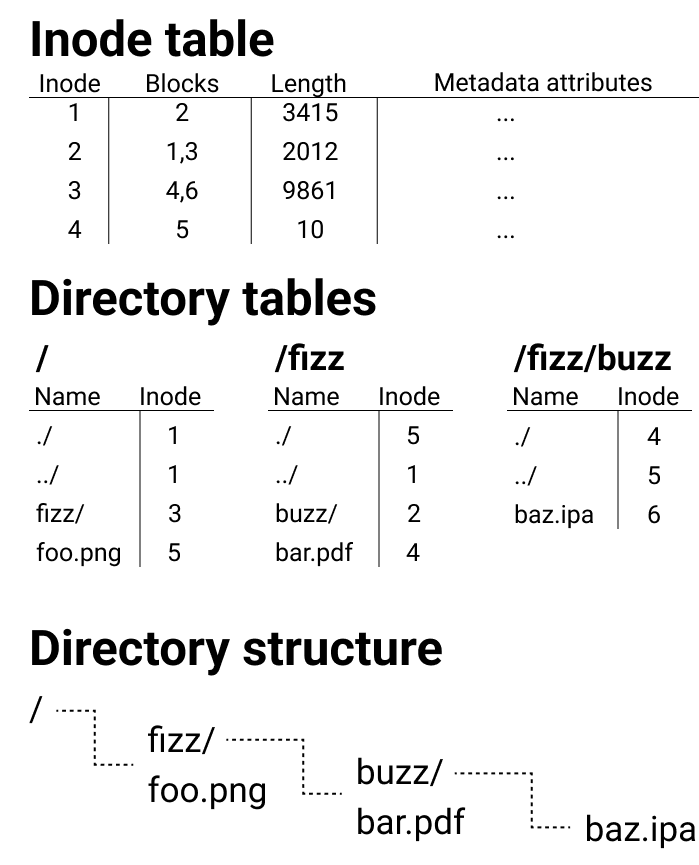
\includegraphics[width=0.8\textwidth]{figures/inode_diagram.png}
	\end{center}
	\caption{Basic structure of inode based filesystem}
	\label{fig:inode_diag}
\end{figure}

Looking at the 4 main file systems of windows, they all have many, sometimes different, functionalities such as links and named streams as well limitations such as a defined theoretical maximum file size\cite{mikbenFileSystemFunctionality}. This is set to 16 exbibytes for NTFS, exFAT and UDF, and for FAT32 it is set to 4 gigabytes. 

\section{Twitter}
\label{sec:twitter}
Twitter is a micro-blog online where users can sign up for a free account and create public posts (tweets) using text, images, and videos. Each post has a unique id associated with it\,\cite{twitterTwitterIDs}. Text posts are limited to $280$ characters while images can be up to \SI{5}{\mega\byte} and videos up to \SI{512}{\mega\byte}\,\cite{MediaBestPractices}. An post with images can contain up to 4 images in one post. There is also a possibility to send private messages to other accounts, where each message can contain up to $10\,000$ characters and the same limitations on files. However, direct messages older than $30$ days are not possible to retrieve through Twitter's API\,\cite{RetrievingOlder302018}. It is possible to create threads of Twitter posts where multiple tweets can be associated in chronological order.

Twitter's API defines technical limits of how many times certain actions can be executed by a user\,\cite{UnderstandingTwitterLimits}. A maximum of $2\,400$ tweets can be sent per day, and the limit is further broken down into smaller limits at semi-hourly intervals. Hitting a limit means that the user account no longer can perform the actions that the limit represents until the time period has elapsed.

\section{Related Work}
\citeauthor{peters_defy_2014} created a deniable filesystem using a log-based structure in \citeyear{peters_defy_2014}\cite{peters_defy_2014}. The filesystem of my project could be seen as a deniable system in the sense that the data is not actually stored on the device, and if the filesystem is not mounted it could be hard to prove that the user actually has data, even if they for instance would find the twitter account. This was also developed using FUSE\cite{noauthor_libfuse_2021} which I also will be using.

% \section{Major background area 1}
% \todo[inline, backgroundcolor=kth-lightblue]{Viktigt bakgrundsområde 1}
There are xxx characteristics that distinguish yyy from other information and communication technology (ICT) system, as shown in Figure~\ref{fig:lotsofstars}. Table \ref{tab:tablecaracteristics} summarizes these characteristics.

 
\begin{figure}[!ht]
  \begin{center}
    
\includegraphics[width=0.5\textwidth]{figures/lots_of_stars.png}
  \end{center}
  \caption{Lots of stars  (Inspired by Figure x.y on page z of [xxx])}
  \label{fig:lotsofstars}
\end{figure}
% \todo[inline, backgroundcolor=kth-lightblue]{Massor av stärnor (Inspirerad av figur x.y på sidan z i [xxx])}


\begin{table}[!ht]
  \begin{center}
    \caption{xxx characteristics}
    \label{tab:tablecaracteristics}
    \begin{tabular}{l|S[table-format=4.6]} % <-- Alignments: 1st column left, 2nd middle, with vertical lines in between
      \textbf{Characteristics} & \textbf{Description}\\
      $\alpha$ & $\beta$ \\
      \hline
      1 & 1110.1\\
      2 & 10.1\\
      3 & 23.113231\\
    \end{tabular}
  \end{center}
\end{table}
% \todo[inline, backgroundcolor=kth-lightblue]{Egenskaper}
% \todo[inline, backgroundcolor=kth-lightblue]{ Beskrivning}

\subsection{Subarea 1.1}
Entangled states are an important part of quantum cryptography, but also relevant in other domains. This concept might be relevant for neutrinos, see for example \cite{kim_small-mass_2016}.

\subsection{Subarea 1.1.2}
Computational methods are increasingly used as a third method of carrying out
scientific investigations. For example, computational experiments were used to
find the amount of wear in a polyethylene liner of a hip prosthesis in \cite{maguire_jr_new_2014}.
…

\subsection{Subarea 1.1.2}
Using the nearest data center may improve performance, see \cite{bogdanov_nearest_2015}


\subsection{Link layer Encapsulation}
\label{sec:llencap}

% See Figure~\ref{fig:ieee8023-data-packet} which uses the \textsf{bytefield}  \LaTeX\ package. 


% \begin{figure}[!ht]
% 	\centering
% \begin{bytefield}{21}
% \bitbox[]{7}{} & \bitbox[]{3}{\tiny octets:} & \bitbox[]{4}{\tiny 6} & \bitbox[]{4}{\tiny 6} & \bitbox[]{3}{\tiny 2} & \bitbox[]{5}{\tiny 46 to 1500} & \bitbox[]{3}{\tiny 0 to 46} & \bitbox[]{2}{\tiny 4}\\ 

% \bitbox[]{8}{\textbf{ETHERNET \\[-1ex] \tiny{data link-layer}}} & \bitbox[]{2}{} & 

% \bitbox{4}{\tiny Destination Address} & \bitbox{4}{\tiny Source Address} & \bitbox{3}{\tiny Length/ Type} & 
% \bitbox{5}{\tiny Data Payload} & \bitbox{3}{\tiny Padding} &
% \bitbox{2}{\tiny CRC} \\

% \bitbox[]{1}{} &\bitbox[]{3}{\tiny octets:} & \bitbox[]{4}{\tiny 7} & \bitbox[]{2}{\tiny 1} & \bitbox[]{0}{$\vdots$ \\[1ex]} & \bitbox[]{16}{} & \bitbox[]{0}{$\vdots$ \\[1ex]} & \bitbox[]{5}{} & \bitbox[]{4}{\tiny Variable}\\

% \bitbox[]{4}{\textbf{MAC \\[-1ex] \tiny{packet}}} & \colorbitbox{lightgray}{4}{\tiny Preamble} & \colorbitbox{lightgray}{2}{\tiny SFD} & \colorbitbox{lightgray}{16}{\tiny MAC Client Data} & \colorbitbox{lightgray}{3}{\tiny Padding} &
% \colorbitbox{lightgray}{2}{\tiny CRC} & \colorbitbox{lightgray}{4}{\tiny Extension}
% \end{bytefield}
%      \label{fig:ieee8023-data-packet}
%      \caption{Ethernet data link layer protocol encapsulated into a IEEE~802.3 MAC packet}
% \end{figure}

\subsection{IP packet headers}
\label{sec:ipheaders}
% The data link layer will receive a packet from the IP layer. The layout of
% an IPv4 packet is shown in Figure~\ref{fig:ipv4-header}. This should be
% contrasted with the IPv6 header shown in Figure~\ref{fig:ipv6-header}.

%
% IPv4 packet header
%
% \begin{figure}[!ht]
% 	\centering
% \begin{bytefield}{32}
% \bitheader{0-31} \\
% \bitbox{4}{\footnotesize{Version}} & \bitbox{4}{IHL} & \bitbox{6}{\tiny{Type of Service}} & \bitbox{2}{{\scriptsize ECN}} \bitbox{16}{Total Length}\\
% \bitbox{16}{Identification} & \bitbox{3}{Flags} & \bitbox{13}{Fragment Offset}\\
% \bitbox{8}{Time to Live} & \bitbox{8}{Protocol} & \bitbox{16}{Header Checksum}\\
% \wordbox{1}{Source Address}\\
% \wordbox{1}{Destination Address}\\
% \colorbitbox{lightgray}{24}{Options} & \colorbitbox{lightgray}{8}{Padding}
% \end{bytefield}
%      \label{fig:ipv4-header} 
%      \caption[IPv4 datagram header]{IPv4 datagram header. Light grey coloured fields are optional.}
% \end{figure}

%
% IPv6 packet header
%
% \begin{figure}[!ht]
% 	\centering
% \begin{bytefield}{32}
% \bitheader{0-31} \\
% \bitbox{4}{\footnotesize{Version}} & \bitbox{8}{Traffic Class} & \bitbox{20}{Flow Label}\\
% \bitbox{16}{Payload Length} & \bitbox{8}{Next Header} & \bitbox{8}{Hop Limit}\\
% \wordbox{4}{Source Address}\\
% \wordbox{4}{Destination Address}\\
% \end{bytefield}
%      \label{fig:ipv6-header}
%      \caption{IPv6 datagram header}
% \end{figure}

\subsection{Test for accessibility of formulas}

As can be seen in these equations:
$c=2 \cdot \pi \cdot r$ or \[ \int_{a}^{b} x^2 \,dx \] a chemical formula: $(C_5O_2H_8)_n$
...

% 
\section{Major background area 2} % \todo[inline, backgroundcolor=kth-lightblue]{Viktigt bakgrundsområde 2}
...
\subsection{\glsentryshort{WLAN} Security}% you can't use the \gls macro in a heading - but you can get the short (\glsentryshort) or long version (\glsentryshort) or \glsentrylong or even the text entry (\glsentrytext) and then there is no problem - see https://tex.stackexchange.com/questions/198140/glossaries-and-custom-section-headings-broken

\section{Related work area} % \todo[inline, backgroundcolor=kth-lightblue]{Relaterade arbeten}


\subsection{Major related work 1} % \todo[inline, backgroundcolor=kth-lightblue]{Relaterade arbeten 1}
Carrier clouds have been suggested as a way to reduce the delay between the users and the cloud server that is providing them with content. However, there is a question of how to find the available resources in such a carrier cloud. One approach has been to disseminate resource information using an extension to OSPF-TE, see Roozbeh, Sefidcon, and Maguire \cite{roozbeh_resource_2013}.


\subsection{Major related work} % \todo[inline, backgroundcolor=kth-lightblue]{Relaterade arbeten}

\subsection{Minor related work 1} % \todo[inline, backgroundcolor=kth-lightblue]{Mindre relaterat arbete 1}


…
\subsection{Minor related work n} % \todo[inline, backgroundcolor=kth-lightblue]{Mindre relaterat arbete n}



% 
\section{Summary} % \todo[inline, backgroundcolor=kth-lightblue]{Sammanfattning}
% \todo[inline, backgroundcolor=kth-lightblue]{Det är trevligt om detta kapitel
%   avslutas med en sammanfattning. Till exempel kan du inkludera en tabell som
%   sammanfattar andras idéer och fördelar och nackdelar med varje - så som
%   senare kan du jämföra din lösning till var och en av dessa. Detta kommer
%   också att hjälpa dig att definiera de variabler som du kommer att använda
%   för din utvärdering.}

% \todo[inline]{It is nice to have this chapter conclude with a summary. For
%   example, you can include a table that summarizes other people's ideas and
%   benefits and drawbacks with each - so as later you can compare your solution
%   to each of them. This will also help you define the variables that you will
%   use for your evaluation.}

\cleardoublepage


\chapter{Method}
\label{ch:methods}

This section presents the methodology of implementing FFS. We also present how the quantitative data used for the evaluation is acquired. Also, the experiments on the filesystems are presented.

\section{FFS}
The artifact that was developed as a result of this thesis is the Fejk FileSystem (FFS). It uses an online web service (\gls{OWS}) to store the data but behaved as a mountable filesystem for the users. The filesystem is a proof-of-concept and does not support all functionalities that other filesystems do, such as links or access permissions. The reasoning is that these behaviors are not required for a useable system, and when comparing FFS to distributed filesystems such as Google Drive, many of these other filesystems also often do not support functionality such as links.

\subsection{Design overview}
FFS uses images to store the data of files, directories and the inode table of the filesystem. These images will are uploaded to the OWS, such as Flickr, as image posts. As mentioned in Section~\ref{sec:ows}, there can be limitations to these posts for certain OWSs. To support file sizes bigger than these limitations, bigger files will be split into multiple posts, requiring FFS to keep track of a list of posts. Figure~\ref{fig:ffs_inode_diag} presents the basic outline of FFS and a example content of the filesystem. FFS is based on the idea of inode filesystems and uses a inode table to store information about the files and directories in the filesystem. However, instead of an inode pointing to specific blocks in a disk, the inode table of FFS will instead keep track of the id numbers of the posts on the OWS where the file or directory is located. The inode table entry for each file or directory will also contain metadata about the entry, such as its size and a boolean indicating if the entry is a directory or not.

\begin{figure}[!ht]
	\begin{center}
	  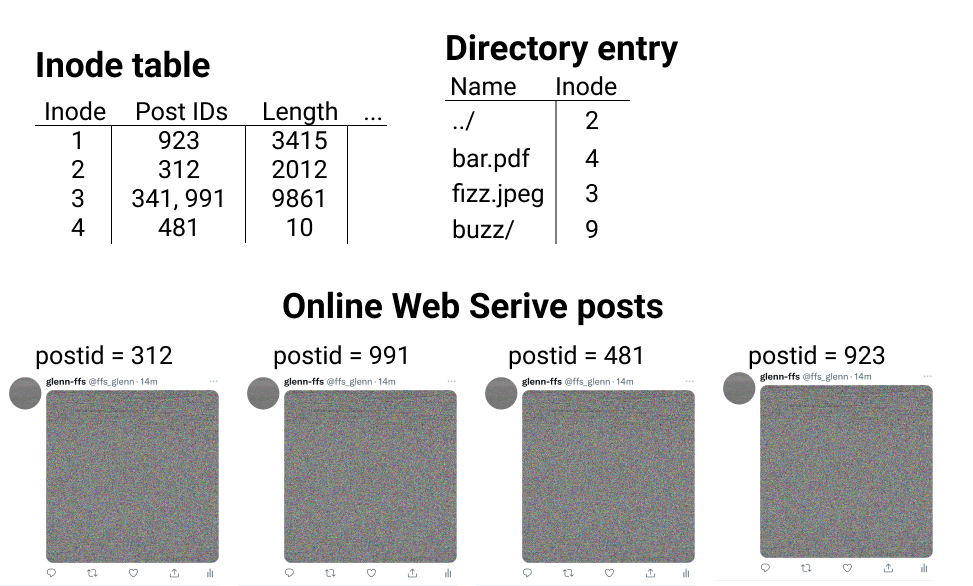
\includegraphics[width=0.8\textwidth]{figures/ffs_inode_diagram.png}
	\end{center}
	\caption{Basic structure of FFS inode-based structure}
	\label{fig:ffs_inode_diag}
\end{figure}

The directories and inode table are represented as classes in C++. Appendix~\ref{app:inode_dir_code} visualizes the main attributes of the \texttt{Directory}, \texttt{InodeTable}, and \texttt{InodeEntry} classes. There can be multiple \texttt{Directory} and \texttt{InodeEntry} objects in the computers' memory and in the filesystem, but there will only exist one \texttt{InodeTable} instance which is relevant. The \texttt{Directory} class is a data structure that stores mappings between filenames and the files' and directories' inode for all files and directories stored in that directory. The \texttt{InodeEntry} is a data structure that keeps track of a file's or directory's information, such as where the data is stored and its metadata, such as size and creation timestamp. The \texttt{InodeTable} stores a mapping between an inode and the files' \texttt{InodeEntry}, and stores all the \texttt{InodeEntry} objects. The \texttt{InodeTable} always has at least one entry which is the root directory. This entry has a constant inode value of 0 for simplicity to look up the root directory. With the help of the root directory, all the files lower in the directory hierarchy can be found. The inode of all files and directories other than the root directory has a unique inode greater than 0. The \texttt{InodeTable} is always the most recent image saved on the OWS, making it easy to find it on the OWS.

To read the content of a known file in a directory has three steps:
\begin{enumerate}
	\item The \texttt{Directory} object of the directory provides the inode of the given filename.
	\item The inode is used to get the \texttt{InodeEntry} from the \texttt{InodeTable}.
	\item Using the inode entry, the the file can be located.
\end{enumerate}
The location of a file or directory is an ordered list of unique IDs of the image posts on the OWS. The data received by downloading these images, decoding them (as described in Subsection~\ref{subsec:file_enc_dec}), and concatenating them, can be read as a file or represented as a \texttt{Directory} object, depending on if the \texttt{InodeEntry} was marked as a file or a directory. 

As directories only know the filenames inode, the \texttt{Directory} object does not have to be saved again (and thus uploaded) when a file or directory in it is edited, for instance adding data. Only the \texttt{InodeEntry}, and thus the \texttt{InodeTable}, needs to be updated with the new post IDs of the new file or directory. This saves computation time as every request to the OWS takes time. However, if the filename is edited or the file or directory is moved to another location, the parent directory of the file or directory would have to be edited, and such its corresponding \texttt{Directory} object has to be updated.

When a new file or directory is created, it is saved in its parent directory with its filename and an inode. The same inode is used in the inode table to keep track of the file's or directory's inode entry. As shown in Appendix~\ref{app:inode_dir_code}, the inode is represented as a unsigned 32-bit integer. The inode is calculated by adding one to the currently greatest inode. This means that new files and directories will always receive a higher greater inode than the ones currently in the inode table. This naïve approach to inode generation does not take in to account that there might be an available inode less than the greatest inode in the inode table (for instance, due to deletion of a previously created file). However, this inode generation approach is fast and will not be a problem until the integer overflows. As the inode is represented using a 32-bit integer, FFS would need to have saved over four billion files before the inode value would overflow. This scenario is not in the scope of this proof-of-concept filesystem.

FFS does not support all filesystem operations that are implementable through FUSE, instead FFS implements a subset of them. The implemented functions are shown in Table~\ref{tbl:fs_impl_op}. The implemented operations are the most vital operations required for a working filesystem\,\cite{kuenningCS135FUSEDocumentation2010}. Operations such as \texttt{chown} provides extended capabilities of the filesystem but these are not required for a proof-of-concept filesystem. The functionality of the filesystem operations implemented by FFS and their implementation details are described in Subsection~\ref{subsec:file_op}. 

\begin{table}[!ht]
	\begin{center}
		\caption{Filesystem operations implementable trough the FUSE API, and wether or not FFS implements them}
		\begin{tabular}{| c | c |}
			
			\hline
			\textbf{Filesystem operation} 	& \textbf{Implemented by FFS}\\
			\hline
			\hline
			\texttt{open} & Yes\\
			\texttt{opendir} & Yes\\
			\texttt{release} & Yes\\
			\texttt{releasedir} & Yes\\
			\texttt{create} & Yes\\
			\texttt{mkdir} & Yes\\
			\texttt{read} & Yes\\
			\texttt{readdir} & Yes\\
			\texttt{write} & Yes\\
			\texttt{rename} & Yes\\
			\texttt{truncate} & Yes\\
			\texttt{ftruncate} & Yes\\
			\texttt{unlink} & Yes\\
			\texttt{rmdir} & Yes\\
			\texttt{getattr} & Yes\\
			\texttt{fgetattr} & Yes\\
			\texttt{statfs} & Yes\\
			\texttt{access} & Yes\\
			\texttt{utimens} & Yes\\
			\texttt{readlink} & No\\
			\texttt{symlink} & No\\
			\texttt{link} & No\\
			\texttt{chmod} & No\\
			\texttt{chown} & No\\
			\texttt{fsync} & No\\
			\texttt{fsyncdir} & No\\
			\texttt{lock} & No\\
			\texttt{bmap} & No\\
			\texttt{setxattr} & No\\
			\texttt{getxattr} & No\\
			\texttt{listxatt} & No\\
			\texttt{ioctl} & No\\
			\texttt{flush} & No\\
			\texttt{poll} & No\\
			\hline

		\end{tabular}
		\label{tbl:fs_impl_op}
	\end{center}
\end{table}

A file, a directory, or the inode table has to be uploaded to the OWS when it is modified to save its current information. As it takes time to make requests to the OWS, FFS is created to make as few requests as possible while still saving the data required. Therefor, only the directory or file that is affected by a change is uploaded to the system, while the ones unaffected can remain the same. The inode table has to be updated with every change of a file or directory as it contains the location of the file or directory.

FFS can be mounted to the local filesystem using FUSE, similar to how you can mount a network drive like an File Transfer Protocol (\gls{FTP}) server. The mounted FFS volume operates similar to any other drive, and can be accessed using, for instance, Apple's Finder or a Z Shell terminal.

\subsection{Cache}
FFS implements a simple in-memory Least Recently Used (\gls{LRU}) cache for the downloaded content. The cache consists of two data structures: 
\begin{itemize}
	\item a Cache Map - a mapping between a post ID and its image data, and
	\item a Cache Queue - a queue keeping track of the cached post IDs.
\end{itemize}
The cache stores a maximum of 20 image posts. The data stored in the cache is the decrypted image data. To avoid FFS to use too much memory, the cache is configured so that images greater than \SI{5}{\mega\byte} are not cached. Each time an image is uploaded or downloaded, it is added to the Cache Map with its post ID as the key. The post ID is also added to the beginning of the Cache Queue. If the Cache Queue exeeds 20 elements, the last elements of the queue is removed, and the corresponding entry in the Cache Map is erased, thus the entry is fully erased from the cache. The queue ensures that the chache is limited to 20 entries, and by using the first in first out valuation method, the queue also ensures that the oldest element in the cache is removed when the cache exeeds the limit. When a file or directory is removed from the filesystem, all its data is also removed from the cache, if it stored there.

Before a post with a specified post ID is downloaded from the OWS, the cache is checked to see if it is storing this post ID. If it is, the stored image is returned. Otherwise, the process continues by downloading the image from the OWS. When the thesis states that a file or directory is downloaded, it is implied that the cache is also checked and the data is possibly returned by the cache instead of requiring to download the data from the OWS.

FFS separately caches both the root directory and the inode table. As both of these data structures are used in many of the filesystem operations, it is important that they can be accessed quickly and not be removed from the cache. Their cache entries are updated when the files are uploaded to the OWS.

\subsection{Encoding and decoding objects}
\label{subsec:file_enc_dec}
Objects that FFS stores, and therefore also encodes and decodes, are: files, directories, and the inode table. All of these objects are stored on the OWS using PNG images with 16 bit RGB color depth. The inode table and the directories are represented as C++ objects in memory during runtime, but are serialized into a binary representation before they are encoded into images. A detailed description of these binary formats is described in Appendix~\ref{app:binary_rep}. The files saved to FFS are also read in to memory in a binary format before being encoded and uploaded to the OWS. 

The input to the image encoder is the binary data do encode as an image. A header (FFS header) is prepended to the binary data, containing among other things, the size of the data and a timestamp of when the data was encoded. The FFS header and the input data is encrypted using authenticated encryption, utilizing GCM and AES. The key used for the encryption is derived using the HKDF function utilizing the SHA-256 hashing algorithm, along with a \SI{64}{\byte} salt vector, re-generated with random data every time new data is being encrypted. The salt is stored with the cipher to ensure that the decryption algorithm uses the same salt to derive the decryption key. The secret used in the HKDF is a password provided by the user. HKDF also uses a initialization vector, re-generated with random data every time new data is being encrypted. The length of the IV is set to 12 bytes. The resulting data from the encryption is the salt, the IV, the encrypted cipher (including the authentication tag). These three data points are concatenated into a string of bytes. This string of bytes is referred to as the Complete Encrypted Data (\gls{CED}).

The dimensions of an FFS image is based on the amount of bytes stored, as described in Section~\ref{sec:data_storage}. The stored data is the CED, prepended with the length of the CED (\gls{LCED}) using 4 bytes. For an image of $X = ceil(\frac{4 + LCED}{6})$ pixels, FFS will set the width $w$ of the image as $w = ceil(\sqrt{X})$. Further, the height $h$ of the image is set as $h = ceil(\frac{X}{w})$. This will require $(w * h) - X$ filler bytes, and will create an image with similar height and width. For certain values of $X$, $h$ will be equal to $w$. For other values of $X$, $h = w-1$. The resulting data encoded in the image is, in order:
\begin{itemize}
	\item 4 bytes representing the LCED,
	\item The CED data, and
	\item Filler bytes
\end{itemize}
The filler bytes are randomized bytes.

The data consisting of the LCED, CED and filler bytes is encoded in to pixel color data for a PNG with 16 RGB bit color depth using the Magick++ library. The result is an image, with a high probability, of what looks like randomized colors for each pixel. This is due to the fact that most pixels are encrypted and therefore the bytes representing this data is seemingly random.

To decode an FFS image, the decoder first interprets the 4 first bytes as the LCED. The salt and IV are retrieved from the CED as they are of known length. The decryption key is derived using the IV and salt, and results in the same key as used in the encryption step because AES is a symmetric cipher algorithm. The remaining bytes of the CED are decrypted using the decryption key. The unencrypted data consists of the FFS header concatenated with the original stored data. The FFS header is asserted to be in the correct format, before the stored binary data is returned from the decryption function. Figure~\ref{fig:file_enc_dec} visualizes the encoder and decoder for all data saved in FFS.

\begin{figure}[!ht]
	\begin{center}
	  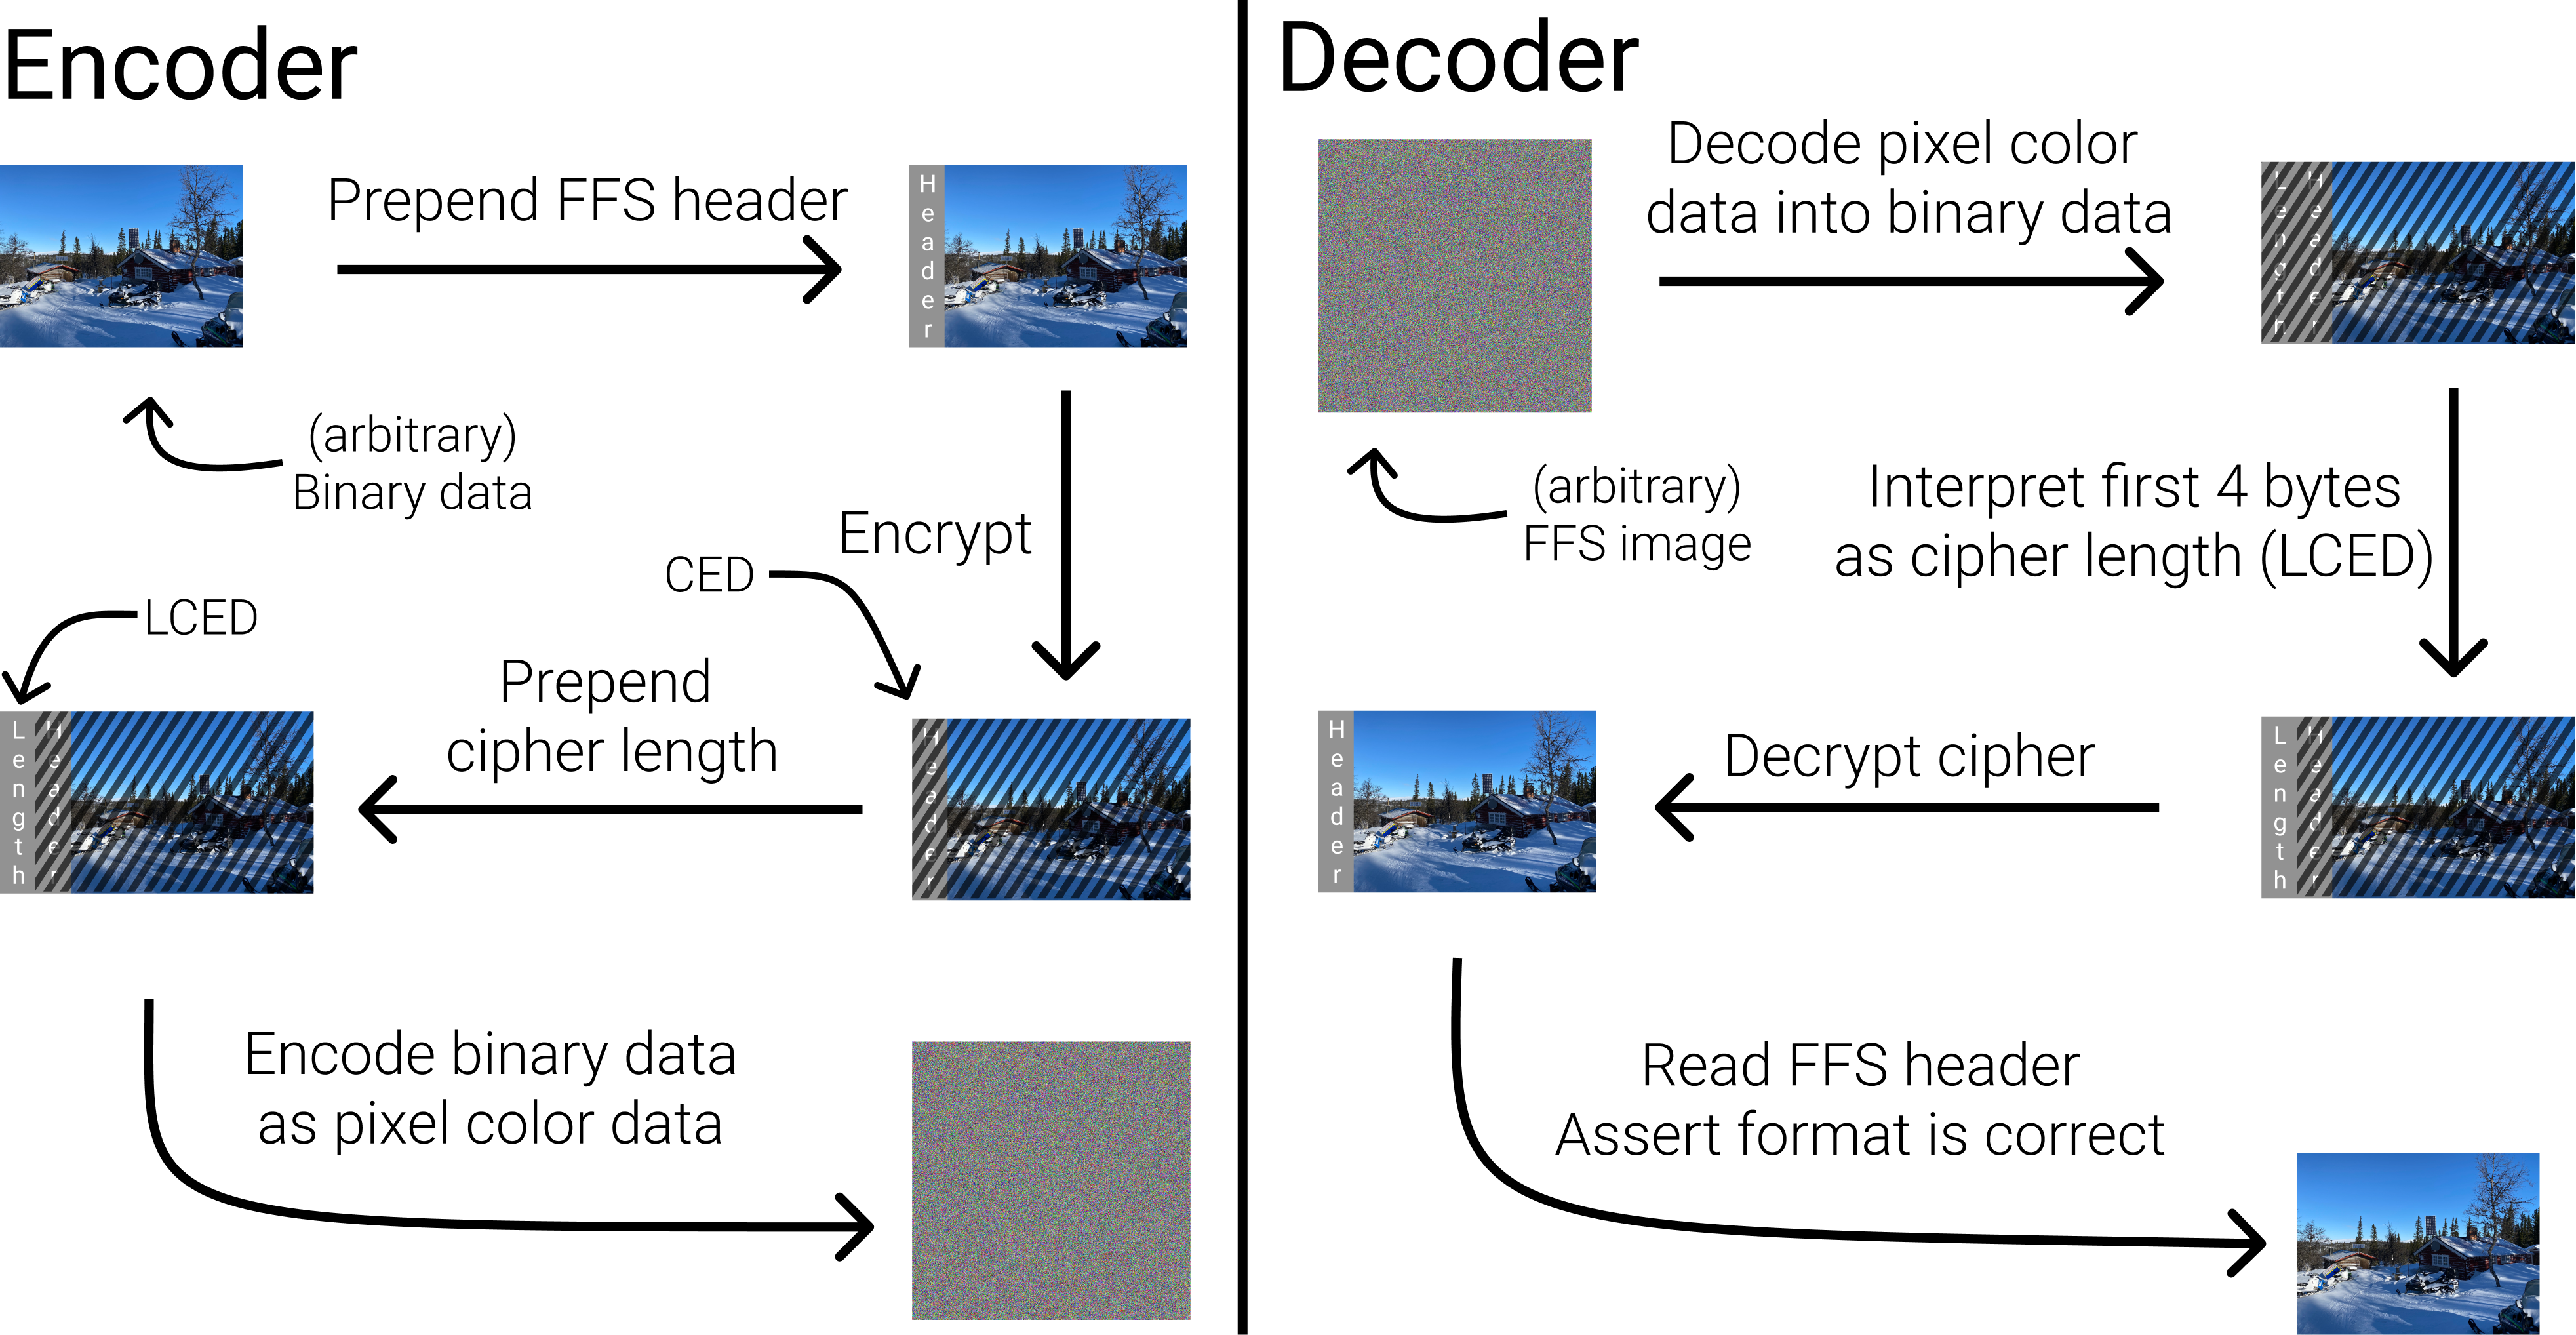
\includegraphics[width=1.0\textwidth]{figures/encoder_decoder.png}
	\end{center}
	\caption[Simple visualization of the encoder and decoder of FFS]{Simple visualization of the encoder and decoder of FFS. The input of the encoder is the binary data to store in FFS, eg. a file, and the output is the FFS image to upload to the OWS. The input to the decoder is an FFS image, and the output is the binary data stored on FFS, eg. a file}
	\label{fig:file_enc_dec}
\end{figure}

The encryption and decryption methods used are state-of-the-art solutions as defined and implemented by Crypto++\,\cite{CryptoLibraryFree}. Crypto++ is a well-used and well maintained C++ library for cryptography, and as of writing has no reported CVE security vulnerabilities for the functionality used by FFS\,\cite{CryptoppSecurityVulnerabilities}.

An FFS image has an upper size limit, defined by the OWS used. This limit is defined further down in this section. If the data to be stored in FFS, such as a file, exceeds this limit, it is split into multiple encoded images. These images will have no association with each other and will be encrypted using different salts and IVs. Only the inode table stores the different post IDs in the order they are encoded in. Files and directories stored in FFS can be separated in to multiple images, however the inode table is limited to only one image for simplicity when interacting with the OWS. This introduces a size limit of the inode table, limiting the filesystem further. More details about the limits are found in Subsection~\ref{subsec:ffs_limits}.

\subsection{Online web services}
As FFS is a proof-of-concept filesystem, it only uses one OWS as its storage medium. However, for a production filesystem, multiple OWSs would be beneficial. This would enable features such as redundancy by using replication over multiple OWSs, for instance in case one OWS would stop working.

The initial intention of FFS was to use Twitter as the OWS. Initial research for the thesis found that it was possible to upload a file and download the same file without any data loss. However, it was later found that this was not a reliable conclusion. Some images uploaded to Twitter were converted to another image format when they were stored by Twitter, which meant that the decoder could not decode the data as it expected another image format. Other images where compressed or recoded which led to data loss when downloading the image. As the decoder of FFS images relies on a specific binary representation of the image, this meant that the images could not be decoded into the previously uploaded data. Twitter has previously publicly announced changes to the way they store images\,\cite{nolanobrienUpcomingChangesPNG2018} and even suggested workarounds\,\cite{nolanobrienFeedbackUpcomingChanges2019} for users who are concerned about the potential data loss. However, during research for the thesis, it was concluded that the workarounds mentioned in \cite{nolanobrienFeedbackUpcomingChanges2019} does no longer work on Twitter. For instance, there have been found PNG images less than 900x900px that have been uploaded, have not been able to be downloaded to the same image, which contradicts the workaround mentioned by the Twitter employee. It is possible that further changes have been made to the data management of images on Twitter, however an official announcement has not been found.

Flickr saves the original version of the uploaded image and thus it can be used to download the same image as was uploaded. This also means that a file that is encoded into an FFS-encoded image can be uploaded, downloaded, and decoded into the same file as before. While they do not assure that they will always support original images, they also do not indicate that this would change. Therefore, Flickr can be used at this moment for the proof-of-concept filesystem that FFS is. A free-tier Flickr account is therefore used for FFS. 

Flickr provides an extensive free REST API for non-commercial use. A user can create applications and generate access tokens for the application. These application tokens are later used to request tokens from users who authenticate using Flickr's web interface, and allow the application to do requests for the user. The application will then receive access tokens for the user, which are used to authenticate with the API for the API calls that require authentication.

Flickr provides the ability to search for all the images posted by a user, and to sort this result by time of posting. Every time an image is uploaded to Flickr, it is due to some modification in the filesystem, for instance a write operation to a file or a creation of a new directory. For every modification in the filesystem, the inode table will have to be updated. Therefore, we can ensure that the inode table is always the most recently uploaded image to Flickr by configuring FFS to upload all other images first, for instance the newly written file. This provides FFS with a simple way of querying the inode table from Flickr - by simply requesting the most recently uploaded image by the Flickr account.

While the Flickr API is extensive in its functionality, FFS only uses a few of the provided capabilities. The Flickr API capabilites that FFS utilizes are:
\begin{itemize}
	\item Upload an image and return the post ID,
	\item Query the most recent image by a user, and return the URL and post ID of the original uploaded image,
	\item Get the URL to the original uploaded image given a post ID, and
	\item Remove an image given a post ID.
	\item Get the image data of the image given its URL
\end{itemize}

For instance, to download the original image given a post ID, two requests are required:
\begin{enumerate}
	\item Getting the URL to the original image using the post ID,
	\item Downloading the image from the URL received from the previous request.
\end{enumerate}

For benchmarking purposes, a fake variant of FFS, Fejk FFS (\gls{FFFS}), has also been developed. FFFS uses a Fake OWS (\gls{FOWS}), which stores the data on the local filesystem. The FOWS is used by FFFS similar to how Flickr is used by FFS, by storing encoded images in it. By storing the images on the local filesystem, the filesystem operations duration is shorter as the local filesystem operations are in general faster than the network requests. This makes it easier to conclude how much of the filesystem operation time is affected by the time of the network requests. The time $T$ of an FFS filesystem operation can be modeled like:
$$
	T = t_{ffs} + t_{ows}
$$
where $t_{ffs}$ is the time that FFS takes to, for example for a file read operation;
\begin{itemize}
	\item to find the file in the inode table,
	\item decode and decrypt the image data,
	\item read the specified amount of data, and,
	\item to output the data
\end{itemize}
This time will be approximately consistent for the same request. However, cache misses/hits in the filesystem and process scheduling can fluctuate the value of $t_{ffs}$. $t_{ows}$ is the total time required to complete all requests to the OWS for a filesystem operation. For instance, for a similar read operation as above;
\begin{itemize}
	\item to download all the directories in the file path,
	\item query the Flickr API for URL pointing to the most recently uploaded image,
	\item download the image representing the inode table, and,
	\item to download the images representing the file to read
\end{itemize}
Depending on the OWS, the latency and bandwidth of the internet connection between the user's machine and the OWS's server can differ a lot. Duplicate requests to the same OWS can also differ significantly due to, for instance, server load balancing and a difference in request quantity from other users at the time of the requests. However, for a FOWS, $t_{ows}$ can be replaced by $t_{fows}$ which will have approximately consistent values for duplicate operations, because the local filesystem is not affected as much by load balancing. The local filesystem requests by other applications on the machine can also be influenced and minimized by not using other applications on the machine while running the benchmarking tool to ensure filesystem requests by the FOWS can be handled quickly by the operating system. However, $t_{fows}$ is affected by, among other things, the underlying storage device of the local filesystem and process scheduling which can still fluctuate the value of $t_{fows}$.

Due to limitations in the library \texttt{Flickcurl} used for uploading images to Flickr, the image to be uploaded to Flickr first has to be saved to the local filesystem. \texttt{Flickcurl} reads the file from disk, before uploading it. Therefore, FFS saves a temporary file on the local filesystem when data is uploaded to Flickr. The temporary file is stored in the \texttt{/tmp} directory of the local filesystem, and is removed directly after the file has been uploaded. However, it is not certain that the operating system removes or overwrites the file data on the storage device, and thus there are ways to recover the deleted data, by for instance adversaries\,\cite{llcsysdevlaboratoriesHowRecoverData2022,cedricAPFSDataRecovery2022,santosHowRecoverData2021}. Although, these methods require you to decrypt the APFS volume, requiring the decryption password. Without this password, the data cannot be recovered. Even with the decryption password, it is not certain that the data is recoverable.

\subsection{Implemented filesystem operations}
\label{subsec:file_op}
Following is a detailed description of all the FUSE operations implemented by FFS, and how they are implemented by FFS. Further explanations about the intended functionality of the operations can be found in \,\cite{kuenningCS135FUSEDocumentation2010}. 

The path of a file is sometimes provided for the filesystem operation and traversed by FFS to understand the requested location. An example path is \texttt{/foo/bar/buz.txt} or \texttt{/foo/bar/baz/}. A path is traversed like the following pseudo code:
\begin{lstlisting}[language=python, caption={Pseudocode of traversing a given path, returning the \texttt{Directory} and the filename}, label=lst:traverse_path,breaklines=true]
# Traverse a given path and return the parent directory object
#  and filename of the path
traverse_path(path) -> (Directory, string):
	# Fetches inode table from the OWS
	inode_table := get_inode_table()
	
	split_path := path.split("/")
	# The filename could be either the name of a file 
	#  or the name of a directory
	filename := split_path.last
	dirs := split_path.remove_last()

	# Get the root dir from cache
	curr_dir = cache.get_root_dir()

	# While there are still directories to traverse,
	#  get the next directory in the list from current
	#  directory
	while(!dirs.empty())
		dir_name := dirs.pop_first()
		inode := curr_dir.inode_of(filename=dir_name)
		inode_entry = inode_table.entry_of(inode=inode)
		# Download the image posts defined by the 
		#  post IDs in the inode entry
		curr_dir = download_as_dir(inode_entry)
	
	return (curr_dir, filename)

\end{lstlisting}

By traversing a path, FFS has to fetch all parent directories in the hierarchy. The file or directory with the filename is not fetched during while traversing the path, as it might not be necessary for the operation. This implies that all operations that relies on the path of the file or directory has to download all parent directories of the path. However, the directories in the path could be cached and therefore not require a download from the OWS. Further, \texttt{open}, \texttt{opendir}, and \texttt{create} can associate a file handle with a file or directory, so that certain other operations can use the file handle instead of traversing the string path. This saves time because the path traversing result is saved in the filesystem state.

After every operation that modifies the inode table, the inode table is uploaded to the OWS and cached. Therefore, it is assumed that the inode table is always up to date in memory and on the OWS. This will be true as long as there are not multiple FFS instances working with the same OWS account at the same time. This scenario has undefined behavior as there is no locking implemented for FFS.

All filesystem operations are synchronous unless specified. Further, FUSE is running in single-thread mode meaning that a filesystem operation call must complete before another can begin. This helps limiting the risk of data races as two processes cannot call different operations that, for instance, modify the inode table at the same time.

\subsubsection{open}
Given a path to a file, the file is associated with a file handle. The file handle is used in subsequent operations to avoid traversing the filepath. The file is not downloaded from the OWS, only the parent directories are downloaded during the path traversing as explained above. An \texttt{open} call must, eventually, be followed by a \texttt{release} call. Although, multiple other operation calls can occur between these events.

\subsubsection{release}
Given a file handle, this operation closes the file in the filesystem, disassociating the file handle with the file. The current states of the file and the inode table are saved to the OWS, and the previous versions of the file and inode table are deleted from the OWS. Subsequent operations for the file will require path traversing as the file handle can no longer be used.

The file must have a file handle associated with it before \texttt{release} is called. This requires a preceding \texttt{open} or \texttt{create} call for the file.

\subsubsection{opendir}
Given a path to a directory, the directory and associated with a file handle. The file handle is used in subsequent operations to avoid traversing the filepath. The directory is not downloaded from the OWS, only the parent directories are downloaded during the path traversing as explained above. An \texttt{opendir} call must, eventually, be followed by a \texttt{releasedir} call. Although, multiple other operation calls can occur between these events.

\subsubsection{releasedir}
Given a file handle, this operation closes the directory in the filesystem, disassociating the file handle with the directory. The current states of the directory and the inode table are saved to the OWS, and the previous versions of the directory and inode table are deleted from the OWS. Subsequent operations for the file will require path traversing as the file handle can no longer be used.

The directory must have a file handle associated with it before \texttt{releasedir} is called. This requires a preceding \texttt{opendir} call.

\subsubsection{create}
This operation creates an empty file in the filesystem given a path, and associates a file handle with the file, similar to \texttt{open}. The empty file will not be uploaded to the OWS as it has no data associated with it. A new entry is added to the parent directory with the filename and a generated inode, and the parent directory is uploaded to the OWS. The new posts representing the parent directory in the OWS is associated with the inode entry of the parent directory in the inode table, and the old posts are deleted in the OWS. An new inode entry is also created in the inode table, representing the new, empty, file.

\subsubsection{mkdir}
This operation creates an empty directory in the filesystem given a path. The directory is not uploaded to the OWS as it has no data associated with it. The parent directory is modified so it is uploaded to the OWS, and the old versions of the parent directory is deleted on the OWS. The parent directory entry in the inode table is modified with the new posts, and a new entry is created for the new directory. The inode table is updated in the OWS.

As opposed to \texttt{create} for files, this operation does not associate a file handle with the directory.

\subsubsection{read}
This operation reads a number of bytes, starting from a set offset, from the file specified by the file handle. The data is read into a provided buffer. The full file is downloaded and read into memory, even if just a small part of the file is requested. The file is also cached so that subsequential requests for the same file are faster. 

\subsubsection{readdir}
This operation reads the filenames inside the directory specified by a file handle. The result includes all filenames in the directory, and the special \texttt{"."} and \texttt{".."} directories.

\subsubsection{write}
This operation writes $s$ bytes, starting at the provided offset $o$, to the existing file at the provided file handle. All the data of the current file is read in to memory. Starting from the offset, the new data overwrites the current data of the file, until $s$ bytes have been written. If $o + s$ is greater than the file's size, the file size is set to $o + s$. If $o + s$ is less than the file's size, the data from position $o + s$ and forward remains the same, and the file size is not modified. See Figure~\ref{fig:write_flow} for a visualization of the result of a \texttt{write} operation given different offsets. The parent directory does not have to modified. 

The file and inode table are not updated to the OWS, this occurs instead in the subsequent \texttt{release} call.

\begin{figure}[!ht]
	\begin{center}
	  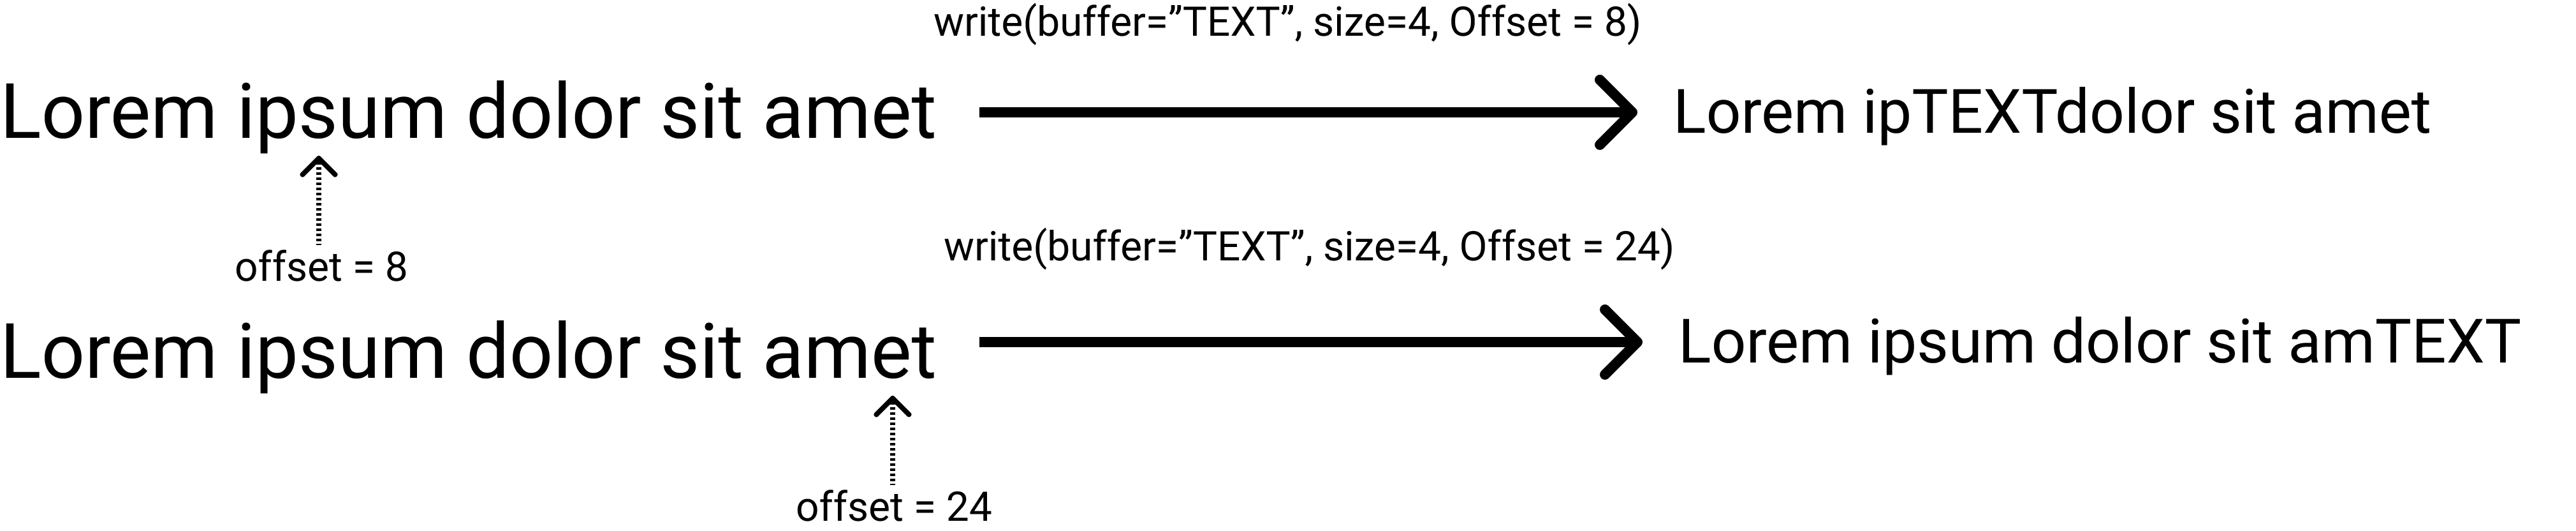
\includegraphics[width=0.9\textwidth]{figures/write_flow.png}
	\end{center}
	\caption{Visualization of how the write operation handles different offsets.}
	\label{fig:write_flow}
\end{figure}

\subsubsection{rename}
This operation renames a file or directory to a new path. Both the old path and the new path have to be traversed to located the parent directories and the file or directory to rename. The file or directory entry in the old parent directory is removed, and the old parent directory is updated to the OWS. A new entry is created in the new parent directory, with the new filename. The new parent directory is updated to the OWS. The inode entry of the renamed file or directory does not have to be modified. However, as both the old parent directories and the new parent directory are updated in the OWS, their inode entries need to be updated with the new posts. The inode table is updated to the OWS and the old table is removed from the OWS. The old posts associated with the old parent directory and the new parent directory are removed from the OWS.

The new path could be in the same directory as the file or directory currently is in. This will not affect the process mentioned above, however the path will only have to be traversed once.

\subsubsection{truncate}
This operation truncates or extends the file in the given path, to the provided size $s$ . The full current file is downloaded into memory. The data of the current file is read into a new buffer until either the file is fully read, or until $s$ bytes have been read. If the current file's size is smaller than $s$, the remaining amount of bytes are added as the NULL character. The new file data is uploaded to the OWS, and the old data is removed from the OWS. The inode table entry is updated with the new posts and uploaded to the OWS. The old inode table is removed from the OWS.

\subsubsection{ftruncate}
This operation is similar to \texttt{truncate}, but is called from a user context which means it has a file handle associated with it. The operation truncates or extends the file in the given file handle, to the provided integer $s$. The full current file is downloaded into memory. The data of the current file is read into a new buffer until either the file is fully read, or until $s$ bytes have been read. If the current file's size is smaller than $s$, the remaining amount of bytes are added as the NULL character.

The file and inode table are not updated to the OWS, this occurs instead in the subsequent \texttt{release} call.

\subsubsection{unlink}
This operation removes a file given the filepath. The file is removed from the parent directory, and the parent directory is updated to the OWS. The old parent directory data is removed on the OWS. The removed file's entry in the inode table is also removed, and the inode table updates the entry for the parent directory with its new posts. The inode table is then updated on the OWS and the old inode table is removed on the OWS. Finally, the data of the removed file is removed from the OWS. The last step is not necessary for a working filesystem; however, to save space on the OWS, this is done. If the OWS permits unlimited images and sizes, this step could be omitted to execution save time.

\subsubsection{rmdir}
Similar to \texttt{unlink}, this operation removes the directory at the path. The directory and all its subdirectories are traversed, and the post IDs of these files and directories are recorded for deletion in the OWS later. Following, the entry of the removed directory is removed from the parent directory. The inode entry for the removed directory is removed. The parent directory is updated to the OWS, and the inode table is updated with the new posts of the parent directory. Following, the inode table is updated to the OWS. The old parent directory and the old inode table are removed from the OWS.

The operation also starts a new thread, where all the posts of files and subdirectories inside the removed directory, are removed from the OWS. This occurs to save space on the OWS, and a separate thread is used to save computation time for subsequent file operations. There is no data race involved as the API is thread safe, and the posts are no longer associated with any data structures on the main thread.

\subsubsection{getattr}
This operations returns attributes about a file or directory given a path. This includes permissions, number of entries (if the provided path points to a directory), and timestamps of creation, last access and last modification. However, as mentioned previously, FFS does not implement all features, such as permissions. Instead of keeping track of a file's or directory's permissions, all calls to valid path will return full read, write, and execute permissions for everyone. However, the timestamps are stored in the inode table of FFS. The file or directory pointed to by the path does not need to be downloaded, all the metadata that FFS stores is accessible through the inode entry in the inode table.

\subsubsection{fgetattr}
This operation is the similar to \texttt{getattr}, but is called from a user program context meaning that the file has a file handle associated with it. Other than skipping the path traverse step, this operation returns the equivalent information as \texttt{getattr}.

\subsubsection{statfs}
This operation returns metadata information about FFS. This includes, among other things, the maximum filename size and the filesystem ID. The operation has a short computation time as it does not have to download or upload any files. The only variable information is read from the inode table which is stored in memory and thus does not have to be downloaded from the OWS.

\subsubsection{access}
This operation, given a path, returns wether or not the path can be accessed. As long as the path is valid, this always returns that it can be accessed.

\subsubsection{utimens}
This operation updates the last access timestamp, the last modified timestamp, or both, of the file or directory at the given path. The file or directory does not have to be downloaded. However, the inode entry for the file's or directory's inode is updated with the new timestamps if they are newer than the previous timestamps but not greater than the current time since epoch. The new state of the inode table is updated to the OWS, and the old version is removed from the OWS.

% \subsection{Unimplemented filesystem operations}
% FIXME: Is this needed? ^ 

\subsection{FFS limitations}
\label{subsec:ffs_limits}
% TODO: Limitations, both in number of bytes, files etc
% Also what it lacks, such as filesystem operations and speed(!)
FFS has numerous of limitations due to both implementation decisions and OWS limits. As Flickr allows a free-tier user account to store up to 1\,000 images of up to \SI{200}{\mega\byte} per image, this allows storage of up to \SI{200}{\giga\byte} of images on per account on Flickr. However, as the inode table is required to be stored on the filesystem, a maximum of 999 images can be used to save file and directory data. This limits the filesystem to a maximum of 999 files and directories when utilizing one free-tier account on Flickr. 

While Flicker supports each image to be up to \SI{200}{\mega\byte}, it is not possible to use the full \SI{200}{\mega\byte} as the file data to store. The image includes, among other things, a PNG header, other PNG attributes, and the CED which in total is of greater size than the unencrypted data. To ensure that the pixel color data along with the PNG header and other PNG attributes does not exceed the limit of \SI{200}{\mega\byte}, FFS limits the pixel color data size to allow at least \SI{10}{\mega\byte} for the PNG header and other PNG attributes, meaning that the pixel color data can be a maximum of \SI{190}{\mega\byte}. The cryptographic variables IV, salt, and the authentication tag are stored in the CED using 12, 16, and 64 bytes respectively, for a total of 92 bytes. The size limit means that these 92 bytes, along with the encrypted cipher text, cannot exceed \SI{190}{\mega\byte}, meaning that the encrypted cipher text cannot exceed $190\,000\,000 - 92 = $\SI{189\,999\,908}{\byte}. However, as AES is a block cipher producing cipher blocks of 16 bytes, the resulting cipher text must be a divisible of 16. The largest encrypted cipher text that FFS allows is therefore $floor(\frac{189\,999\,906}{16})*16 = 189\,999\,904$ bytes. Due to plain text padding, the unencrypted plain text can be a maximum of one byte less than this value\,\cite{z.z.coderAnswerSizeData2010}, meaning that the plain text can be a maximum of \SI{189\,999\,903}{\byte}. For simplicity, this is rounded down to \SI{189}{\mega\byte}, leaving almost \SI{11}{\mega\byte} in total for the PNG header and other PNG attributes. \SI{189}{\mega\byte} is set as the maximum amount of data FFS will store per image. Data greater than \SI{189}{\mega\byte} is split into multiple encoded images. For instance, a file of \SI{200}{\mega\byte} will be stored as \SI{189}{\mega\byte} in one image, and \SI{11}{\mega\byte} in another. 

\SI{189}{\mega\byte} of usable data per images gives FFS a maximum storage capacity of \SI{188.811}{\giga\byte} using one free-tier account on Flickr. Each file with data requires at least one image, thus there can be a maximum of 998 non-empty files and directories in the filesystem, excluding the root directory. However, there could also be just one single file of \SI{188.811}{\giga\byte} stored in the filesystem.

The inode table also keeps information about empty files and directories even though they store no data on the OWS. The inode of a file or directory is an unsigned 32-bit integer, meaning that the inode table could theoretically store up to over four billion files and directories. However, due to the constraints mentioned above, most of these files and directories would have to be empty as Flickr limits the amount of images stored. An empty file requires \SI{37}{\byte} in the inode table. As the inode table is limited to one single image on the OWS, the inode table is limited to a maximum size of \SI{189}{\mega\byte}. Further, the size of the inode table is \SI{4}{\byte} plus the size of each entry, and one of these entries is the root directory. Even if a file is empty, it is still stored with its filename and inode in its parent directory. A non-empty directory in the inode table requires approximately (depending on the post ID length generated by the OWS) \SI{12}{\byte} per file or directories it contains. The maximum number of empty files and directories $X$ that the inode table can store is therefore, approximately:
$$
	X = ceil(\frac{189\,000\,000 - 4 - (12 * X)}{37}) + 1, X = 3\,857\,143
$$
The additional directory is the root directory. Thus, the maximum number of files and directories that the inode table can store is close to four million, however this requires all files and directories, except the root directory, to be empty. These calculations are based on a single free-tier Flickr account. However, a future expansion of FFS could include multiple user accounts, and multiple services. This could increase the limits on the filesystem.

Limits to the file sizes also depend on the machine where FFS is mounted. When a file is read or written to, the complete file is read into memory. This requires the computer to provide at least as much memory as the size of the file. However, even if the computer has less memory available, more memory can often be provided through memory swap on the hard disk. Apple ensures that the swapped data is securely encrypted on the hard disk\,\cite{appleinc.WhatSecureVirtual}. However, using memory swap puts a constraint on the storage of the computer to be sufficient. Also, as FFS temporarily saves the data on the local filesystem before it is uploaded to Flickr, the storage device must have sufficient storage available. For instance, a file larger than the available storage on the local filesystem cannot be saved to FFS. If the local filesystem has no available storage, very few filesystem operations can be performed on FFS as any operation that modify the inode table requires the new inode table to be saved to the local filesystem before it is uploaded to Flickr. 

A limitation of FFS that is not possible to quantify is the bandwidth and latency of the network connection from the user to Flickr. The connection can vary significantly depending on for instance the network load in a given moment and the geographic location of the user. A slow network connection is not something FFS can solve, but is left as an exercise for the reader.

\cleardoublepage

\chapter{What you did} % \todo[inline]{Choose your own chapter title to describe this}
\label{ch:whatYouDid}
% \todo[inline, backgroundcolor=kth-lightblue]{[Vad gjorde du? Hur gick det till? – Välj lämplig rubrik (“Genomförande”, “Konstruktion”, ”Utveckling”  eller annat]}


% \todo[inline]{What have you done? How did you do it? What design decisions did you make? How did what you did help you to meet your goals?}
% \todo[inline, backgroundcolor=kth-lightblue]{Vad du har gjort? Hur gjorde du det? Vilka designval gjorde du?\\
% Hur kom det du hjälpte dig att uppnå dina mål?}

% the following sets the TOC entry to break after the & - note you have to include the first letter of the following word as it get swolled by the \texorpdfstring{}{} processing
\section[Hardware/Software design …/Model/Simulation model \&\texorpdfstring{\\}{ p} parameters/…]{Hardware/Software design …/Model/Simulation model \& parameters/…}
% \todo[inline, backgroundcolor=kth-lightblue]{Hårdvara / Mjukvarudesign ... / modell / Simuleringsmodell och parametrar / …}

Figure~\ref{fig:homepageicon} shows a simple icon for a home page. The time
to access this page when served will be quantified in a series of
experiments. The configurations that have been tested in the test bed are
listed in Table~\ref{tab:configstested}.

% \todo[inline, backgroundcolor=kth-lightblue]{Figur~\ref{fig:homepageicon}  visar en enkel ikon för en hemsida. Tiden för att få tillgång till den här sidan när den laddas kommer att kvantifieras i en serie experiment. De konfigurationer som har testats i provbänk listas ini tabell~\ref{tab:configstested}.\\
% Vad du har gjort? Hur gjorde du det? Vilka designval gjorde du?}
 
\begin{figure}[!ht]
  \begin{center}
    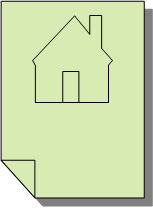
\includegraphics[width=0.25\textwidth]{figures/Homepage-icon.png}
  \end{center}
  \caption{Homepage icon}
  \label{fig:homepageicon}
\end{figure}

\begin{table}[!ht]
  \begin{center}
    \caption{Configurations tested}
    \label{tab:configstested}
    \begin{tabular}{l|c} % <-- Alignments: 1st column left, 2nd middle and 3rd right, with vertical lines in between
      \textbf{Configuration} & \textbf{Description} \\
      \hline
      1 & Simple test with one server\\
      2 & Simple test with one server\\
    \end{tabular}
  \end{center}
\end{table}
% \todo[inline, backgroundcolor=kth-lightblue]{Testade konfigurationer}

\section{Implementation …/Modeling/Simulation/…}
\label{sec:implementationDetails}
% \todo[inline, backgroundcolor=kth-lightblue]{Implementering … / modellering / simulering / …}


\subsection{Some examples of coding}

Listing~\ref{lst:helloWorldInC} shows an example of a simple program written
in C code.

\begin{lstlisting}[language={C}, caption={Hello world in C code}, label=lst:helloWorldInC]
int main() {
printf("hello, world");
return 0;
}
\end{lstlisting}


In contrast, Listing~\ref{lst:programmes} is an example of code in Python to
get a list of all of the programs at KTH.

\lstset{extendedchars=true}
\begin{lstlisting}[language={Python}, caption={Using a python program to
    access the KTH API to get all of the programs at KTH}, label=lst:programmes]
KOPPSbaseUrl = 'https://www.kth.se'

def v1_get_programmes():
    global Verbose_Flag
    #
    # Use the KOPPS API to get the data
    # note that this returns XML
    url = "{0}/api/kopps/v1/programme".format(KOPPSbaseUrl)
    if Verbose_Flag:
        print("url: " + url)
    #
    r = requests.get(url)
    if Verbose_Flag:
        print("result of getting v1 programme: {}".format(r.text))
    #
    if r.status_code == requests.codes.ok:
        return r.text           # simply return the XML
    #
    return None
\end{lstlisting}


\cleardoublepage


\chapter{Results and Analysis}
\label{ch:resultsAndAnalysis}


\cleardoublepage


\chapter{Discussion}
\label{ch:discussion}
The benchmarking results presented in the previous chapter are analyzed and discussed in Section~\ref{sec:dis_fs}. Furthermore, \gls{FFS}'s deniability and security are analyzed and discussed in Section~\ref{sec:dis_sec}. Potential societal and environmental impacts of \gls{FFS} are presented in Section~\ref{sec:imp}.

% \todo[inline, backgroundcolor=kth-lightblue]{Diskussion\\
% Förbättringsförslag?}
% \todo[inline]{This can be a separate chapter or a section
%   in the previous chapter.}

\section{Filesystems}
\label{sec:dis_fs}
Figure~\ref{fig:bench_ffs_read}, Figure~\ref{fig:bench_ffs_re_read}, and Figure~\ref{fig:bench_ffs_rnd_read} show that \gls{FFS} performs poorly for Read operations with a small buffer size. Beginning at \SI{4}{\kilo\byte} buffer size, the performance in general increases with the first few buffer sizes. This indicates that the overhead of the \gls{FFS} read operation is high as the performance gets better when it reads fewer buffers. Overhead of the read operation includes, among other things, the time to fetch the image from Flickr if it is not in the cache, and decrypting the image which is required even if the image is cached. Further, it is expected that \mbox{Re-Read} performs better than Read when the file size is small enough to fit in the cache. This is also a conclusion that can be drawn from the result. However, looking at Figure~\ref{fig:bench_ffs_read}, and Figure~\ref{fig:bench_ffs_re_read}, we can also see that \mbox{Re-Read} overall performs better for file sizes bigger than the \SI{5}{\mega\byte} cache file size limit as well. Especially for the file sizes \SI{32\,768}{\kilo\byte} to \SI{262\,144}{\kilo\byte}, the performance of the Read test is in general very low. As Figure~\ref{fig:res_box_read} and Figure~\ref{fig:res_box_reread} shows, the average performance of \mbox{Re-Read} is more than double than the average performance of Read for \gls{FFS}. It is expected that the cache will increase the performance of the filesystem. The reason that \mbox{Re-Read} performs better than the Read test for files bigger than the cache size limit could be due to a cache in Flickr. It is possible that Flickr prepares often-requested images in a cache that serves the image faster than less-requested images. This could influence the time required to get the image from Flickr. It is also possible that IOZone does not close the file before it is read again, meaning that the file can be kept in memory as \gls{FFS} caches open files that have been read. IOZone does not specify when the file is closed.  Random Read also performs better than the Read test for big file sizes. This could also be because the file has not been closed since the file was read in to memory, enabling \gls{FFS} to provide the requested data faster. However, if the file would not be closed after a write test, the write test of \gls{FFS} should have the same performance as the write test of \gls{FFFS} as neither of the two filesystems actually save the data in their storage medium until the file has been closed. As the write tests of \gls{FFS} and \gls{FFFS} are not very similar, it is improbable that the file is not closed after the write tests. Furthermore, as the write tests are performed before the read tests, there is no possibility that the file was kept open after a read test either.

While the \mbox{Re-Read} and Random Read tests increases in performance for the first buffer sizes, the performance also decreases eventually. Looking at the data presented in Figure~\ref{fig:bench_ffs_re_read} and Figure~\ref{fig:bench_ffs_rnd_read}, the buffer sizes \SI[per-mode = symbol]{4\,096}{\kilo\byte} to \SI[per-mode = symbol]{16\,384}{\kilo\byte} have, in general, lower performance than the buffer sizes \SI[per-mode = symbol]{256}{\kilo\byte} to \SI[per-mode = symbol]{2\,048}{\kilo\byte}, for the same file size. This indicates that the optimal buffer size for \gls{FFS} read operations on previously read files is not the biggest possible buffer size, but rather around \SI[per-mode = symbol]{512}{\kilo\byte}, depending on the file size. The biggest file size has its best performance for a buffer size of \SI[per-mode = symbol]{512}{\kilo\byte}. Looking at the \SI[per-mode = symbol]{131\,072}{\kilo\byte} file size, it peaks for both the \mbox{Re-Read} test and the Random read test at \texttt{buffer size = 128\,kB}, and its performance for that buffer size for both tests are higher than any other performance of any file size or buffer size in both tests, for the filesystem. This is interesting because the \SI[per-mode = symbol]{131\,072}{\kilo\byte} file size does not always outperform the other file sizes. Looking at the \mbox{Re-Read} test, the \SI[per-mode = symbol]{262\,144}{\kilo\byte} has the best performance for seven of the 13 tests while the \SI[per-mode = symbol]{131\,072}{\kilo\byte} file size has the best performance for five buffer sizes, namely the first one, the last three and for \texttt{buffer size = 128\,kB}. The \SI[per-mode = symbol]{16\,384}{\kilo\byte} file size has the best performance of the test once, for \texttt{buffer size = 1\,024\,kB}. Considering how fast the operations actually are, it is possible to understand why the values can fluctuate. For instance, the \mbox{Re-Read} test for \gls{FFS} using \texttt{file size = 16\,384\,kB, buffer size = 1\,024\,kB} has a performance of \SI[per-mode = symbol]{7\,599\,353}{\kilo\byte\per\second}. Transferring \SI[per-mode = symbol]{16\,284}{\kilo\byte} at \SI[per-mode = symbol]{7\,599\,353}{\kilo\byte\per\second} takes \SI[per-mode = symbol]{2.14}{\milli\second}. If it would take 10\% more time, the performance would instead be under \SI[per-mode = symbol]{7\,000\,000}{\kilo\byte\per\second}, meaning that the \SI[per-mode = symbol]{262\,144}{\kilo\byte} file size would have better performance for the same buffer size. However, if it instead would take 10\% less time to perform the \texttt{file size = 16\,384\,kB, buffer size = 1\,024\,kB} \mbox{Re-Read} test, it would reach a performance of \SI[per-mode = symbol]{8\,443\,725.6}{\kilo\byte\per\second} which would be the highest performance of the test on \gls{FFS} of all file sizes and buffer sizes. Small time differences can significantly affect the performance of the tests. The time of the filesystem operations can be fluctuated by process scheduling and the internet connection, among other things.

The performance of the write operations of \gls{FFS} are highly influenced by the file size. As shown in Figure~\ref{fig:bench_ffs_write}, Figure~\ref{fig:bench_ffs_re_write}, and Figure~\ref{fig:bench_ffs_rnd_write}, bigger file sizes implicates better performance for the write operations, generally. The best performing file size was most often the largest file size, \SI[per-mode = symbol]{262\,144}{\kilo\byte}. Furthermore, the biggest file size of the tests perform better for the Write test than for the \mbox{Re-Write} and Random Write test. This is interesting as the Write test includes the overhead of creating the files before writing to them, which \mbox{Re-Write} and Random Write does not.

One interesting comparison is between the benchmark results of \gls{FFS} and \gls{GCSF}. Both filesystems are \mbox{cloud-based} \gls{FUSE} filesystems dependent on an internet connection to their respective storage servers. Looking at the box plots in Section~\ref{sec:res_bench}, we can see that \gls{GCSF} outperforms \gls{FFS} in both average performance and median performance for all tests. However, \gls{GCSF} does not have any data for the biggest file size while \gls{FFS} has data for it. Looking at Figure~\ref{fig:bench_ffs_re_read} and Figure~\ref{fig:bench_gcsf_re_read}, we can see that \gls{FFS} performs better than \gls{GCSF} for many of the bigger file sizes for the \mbox{Re-Read} test. It is possible that \gls{FFS} would perform better than \gls{GCSF} for the \SI{262\,144}{\kilo\byte} file size test if \gls{GCSF} could run the test. However, even if that would be the case, it is also possible that \gls{GCSF} would still perform better overall. One reason that \gls{GCSF} generally outperforms \gls{FFS} could be because the \gls{FFS} cache stores the encrypted version of the image, meaning that before the data is read, the image must first be decrypted and decoded. As Google Drive provides the raw data of the file stored, \gls{GCSF} can store the raw data in its cache meaning that the data in the read operation can be returned faster. If Google Drive caches the raw file data as well, it does not have to decrypt the data when serving it to \gls{GCSF}. \gls{GCSF} also outperforms \gls{FFS} in all the write tests. The reason could be that \gls{GCSF} does not have to encrypt the data nor encode it as images. This could save significant computation time. The average (reference point) bandwidth measured when the two filesystem benchmarks were run are similar, indicating that there was not a big difference in the internet connection to the measurement servers. However, as this does not measure the actual internet connection to the \gls{OWS}, the actual bandwidth of the filesystem could be different from this value. However, even assuming that the bandwidth of the internet connections of \gls{GCSF} and \gls{FFS} are equal, \gls{GCSF} can still benefit from fewer REST \gls{API} calls. As Google Drive is a filesystem, the inode table of the filesystem, or however the filesystem is organized, can be stored on the service without exposing it to the user. For instance, assuming that Google Drive uses an inode table like \gls{FFS}, the inode table would never have to be downloaded and uploaded by \gls{GCSF}. By simply uploading a file and specifying what its path and filename is, the inode table does not have to be modified by the user but can be handled by Google Drive in the background, potentially after the request has completed requiring less time for the file upload request. Meanwhile, \gls{FFS} has to upload the inode table after every file modification. Additionally, the old version of the file and inode table must be removed. This requires \gls{FFS} to perform at least four requests for all modifications:
\needspace{5\baselineskip}
\begin{itemize}
	\item Upload a new image with the new file content,
	\item Upload a new image with the new inode table content,
	\item Remove the old file, and,
	\item Remove the old inode table
\end{itemize}
Although, removing the old images is performed on another thread. Meanwhile, uploading a modified file to Google Drive requires one \gls{API} request using the file's ID\,\cite{FilesUpdateDrive2022} which will perform the same functionality as the four requests required for \gls{FFS}. The ID of the file could be stored locally in memory by \gls{GCSF} to be able to serve file ID's quickly, but this data structure does not have to be uploaded to Google Drive. Furthermore, when downloading a file, parts of the file can be downloaded rather than the full file\,\cite{googleDownloadFilesDrive2022}. This can reduce the time as the full file does not have to be downloaded every time a file is read. Even if we could download parts of a file from Flickr for \gls{FFS}, it would not make sense as we need the full file content to decrypt it. Futhermore, with Google Drive's 800 million daily users\,\cite{lardinoisGoogleUpdatesDrive2017} versus Flickr's 60 million monthly users\,\cite{campbellFlickrStatistics20222022}, Google Drive is a much bigger service. This could mean that it has better infrastructure which can process uploaded data faster than Flickr can.

Certain data points in the graphs presented in Section~\ref{sec:res_bench} are outliers from groups of data points. For instance, looking at the \mbox{Re-Read} test for \gls{GCSF} in Figure~\ref{fig:bench_gcsf_re_read} for \texttt{file size = 32\,768\,kB, buffer size = 256\,kB}, the test data point has much lower performance than the the other data points for similar buffer sizes in the same test with the same file size. There are many possible reasons behind this drop in performance. One reason could be a slow internet connection to Google Drive in the point of time when the specific data point was benchmarked, for instance due to a higher load of other user requests to the service. Due to the \gls{OWS} being an external service that other users use at the same time, it is always possible that the \gls{OWS} of the \mbox{cloud-based} filesystems experiences a high \mbox{user-demand} at any time. Another reason of the data outlier can also be because the operating system scheduler scheduled the \gls{GCSF} process unfavorable at that time. This is an especially possible reason to the outlier data points for the \mbox{non-cloud-based} filesystems \gls{FFFS} and \gls{APFS}. For instance, Figure~\ref{fig:bench_apfs_rnd_read} shows two outliers for \texttt{file size = 131\,072\,kB}, namely \texttt{buffer size = 4\,096\,kB} and \texttt{buffer size = 8\,192\,kB}. They could also have lower performance due to disk scheduling and cache management. The cached files could be removed from the cache if other processes are reading other files from the disk at the same time, invalidating the cache of the benchmark file.

Other outlier data points have much higher performance than the other data points in a test. For instance, looking at the Write test for \gls{FFFS} in Figure~\ref{fig:bench_fffs_write}, there are data points for \texttt{file size = 8\,192\,kB}, \texttt{file size = 16\,384\,kB}, and \texttt{file size = 32\,768\,kB} that have much higher performance than the other data points. While most data points are approximately between \SI[per-mode = symbol]{6\,500}{\kilo\byte\per\second} to \SI[per-mode = symbol]{8\,300}{\kilo\byte\per\second}, two of these file sizes have one outlier, and one has two outliers, of approximately \SI[per-mode = symbol]{100\,000}{\kilo\byte\per\second}. Outliers can also be seen in Figure~\ref{fig:bench_fffs_re_write} and Figure~\ref{fig:bench_fffs_rnd_write} for the \mbox{Re-Write} and Random Write tests on \gls{FFFS}. \gls{FFFS} is not a cloud-based filesystem and is therefore not affected by a fluctuating internet connection. Rather, this is possibly the result of favorable process scheduling and disk operation scheduling. As both file sizes exceed the cache limit of \gls{FFFS}, the cache of the filesystem should not affect the value. However, it is a possibility that IOZone did not close the file or that the \texttt{close} operation was not performed correctly for the preceding test, which would keep the open file in memory regardless of size. This would result in faster file operation as the file would not have to be read from the disk. Furthermore, if the \texttt{close} operation was not called for a test, the filesystem would not write the data to the disk resulting in shorter execution time, leading to a higher performance. Therefore, if there was a missed \texttt{close} operation, the following test or preceding test should also have higher performance than the other data points. However, looking at, for instance, the preceding Read test for \texttt{file size = 32\,768\,kB}, buffer size = 2\,048\,kB in Figure~\ref{fig:bench_fffs_read} and the subsequent \mbox{Re-Read} test for \texttt{file size = 32\,768\,kB, buffer size = 2\,048\,kB} in Figure~\ref{fig:bench_fffs_re_read}, those data points are not outliers which indicates that it the outlier in the Write test probably is not due to a missed \texttt{close} call.

Comparing \gls{FFFS} benchmarking results against the \gls{APFS} benchmarking results, we can compare the theoretical best performance of \gls{FFS} against a \mbox{general-purpose} \mbox{widely-used} filesystem. Furthermore, we can compare \gls{FFFS} against the underlying filesystem in which it is storing its data. In Figure~\ref{fig:bench_fffs_read} and Figure~\ref{fig:bench_apfs_read} we can see that the read operation perform similarly for \gls{FFFS} and \gls{APFS}, where \gls{APFS} is in general faster than \gls{FFFS}. However, for certain data points, such as \texttt{file size = 131\,072\,kB, buffer size = 256\,kB}, \gls{FFFS} has higher performance than \gls{APFS} with \SI[per-mode = symbol]{7\,525\,973}{\kilo\byte\per\second} for \gls{FFFS} and \SI[per-mode = symbol]{5\,927\,107}{\kilo\byte\per\second} for \gls{APFS}. As the file size is bigger than \SI{5}{\mega\byte} it was not stored in the cache of \gls{FFFS} and the filesystem therefore had to read it from \gls{APFS}. The reason why \gls{FFFS} outperformed \gls{APFS} at this data point is therefore most likely due to process scheduling or because the buffer size used by the test is less efficient for \gls{APFS} than the one called on \gls{APFS} by \gls{FFFS}. The buffer size used by \gls{FFFS} to read the file from \gls{APFS} is not certain to be the same as \gls{FFFS} was called with. The buffer size used by \gls{FFFS} on \gls{APFS} is set by the implementation of \texttt{basic\_filebuf}\,\cite{cppreference.comStdBasicFilebuf2020}.

The cache of a filesystems can generally influence the performance of the read operations. However, there is no significant drop in performance for \gls{FFFS} when reading a file that fits in the \gls{FFFS} cache, and one that does not. In fact, the performance of the Read test for \texttt{file size = 8\,192} is in general better than for \texttt{file size = 4\,096} and \texttt{file size = 2\,048} on \gls{FFFS}, even though the \SI{8\,192}{\kilo\byte} file cannot fit in the \gls{FFFS} cache while the other file sizes can, as long as the encrypted data and the PNG attributes do not make the file bigger than \SI[per-mode = symbol]{5}{\mega\byte}. The reason why these files can be provided fast is most probably due to the kernel caching of the files. However, the performance does drop significantly for \texttt{file size = 262\,144\,kB} compared to the previous file sizes, indicating that these files were not be cached by the kernel. The reason to this could be that \gls{FFFS} has to save the data as two images rather than one as the image size limit of \gls{FFFS} is the same as the limit for \gls{FFS}. All files that are read from \gls{FFFS} that are not in any cache are read from disk, which invokes at least one \gls{APFS} read operation. While the \gls{APFS} read operation called might not be called with the same buffer size as the read operation called by IOZone on \gls{FFFS}, the performance of the \gls{FFFS} read operation cannot exceed the \gls{APFS} read operation. However, the similarity of the performance between \gls{FFFS} and \gls{APFS} indicates that \gls{FFS} implements small read operation overhead, and that the read operation performance of \gls{FFS} depends to a great extent on the internet bandwidth and latency to the \gls{OWS}, as well as the \gls{OWS}'s data processing performance.

The only implementation difference between \gls{FFS} and \gls{FFFS} is that \gls{FFS} stores the produced images on Flickr while \gls{FFFS} stores the produced images on the local filesystem. Therefore, the time difference of an \gls{FFS} operation compared to an \gls{FFFS} operation should only depend on the internet connection to Flickr and how fast Flickr can process the requests. For instance, looking at the Write tests for the two filesystems, \gls{FFFS} outperforms \gls{FFS} significantly. Looking at one file size, for instance, \texttt{file size = 8\,192} \gls{FFFS} has an average performance of approximately \SI[per-mode = symbol]{15\,800}{\kilo\byte\per\second} and \gls{FFS} has an average performance of approximately \SI[per-mode = symbol]{1\,050}{\kilo\byte\per\second} for the Write test. This means that the test took on average \SI{518}{\milli\second} for \gls{FFFS} and \SI{7\,802}{\milli\second} for \gls{FFS}. The same test for the same file size for \gls{APFS} had an average performance of \SI[per-mode = symbol]{612\,000}{\kilo\byte\per\second}, meaning it took on average \SI[per-mode = symbol]{133}{\milli\second} for \gls{APFS} to save the \SI[per-mode = symbol]{8\,192}{\kilo\byte} file. Subtracting this value from the test time of \gls{FFFS}, we get the average overhead of the Write test for both \gls{FFS} and \gls{FFFS} as they have the same overhead. The time the test takes for \gls{FFFS} is the same as the time the test takes for the Write overhead plus the time \gls{APFS} takes to save the file. The average overhead time of the Write test for \gls{FFS} and \gls{FFFS} is therefore \SI[per-mode = symbol]{385}{\milli\second}, meaning that the requests and the request's overhead by \gls{FFS} took on average $7\,802 - 385 =$ \SI{7417}{\milli\second} which is about 95\% of the computation time for this test. Assuming the upload bandwidth to Flickr is the measured reference bandwidth of \gls{92.95}{\mega\byte\per\second}, uploading \SI[per-mode = symbol]{8\,192}{\kilo\byte} would take \SI[per-mode = symbol]{705}{\milli\second}. This means that the remaining \SI[per-mode = symbol]{6\,712}{\milli\second} were used for request overhead, such as preparing for the request, waiting for Flickr to process the data, and receiving the response from Flickr, including the post ID. This indicates that with faster data processing by Flickr, \gls{FFS} could potentially be faster. Furthermore, it indicates that the bandwidth of the internet connection to the \gls{OWS} is not the most important factor of the performance of \gls{FFS}. Even if uploading the file over the internet to the \gls{OWS} would be instant, it would reduce the file operation time by less than 10\%. To improve the filesystem operation performance, using a \gls{OWS} which can process the data faster is of more importance. The calculations above assume that the bandwidth to Flickr was approximately the same as the bandwidth to the measurement servers. It is possible that the bandwidth to Flickr was much lower, which would mean that the bandwidth has more impact of the filesystem operation time.

Looking at the same file size for the Read test, \gls{FFFS} has an average performance of approximately \SI[per-mode = symbol]{4\,804\,000}{\kilo\byte\per\second} and \gls{FFS} has an average performance of approximately \SI[per-mode = symbol]{4\,234\,000}{\kilo\byte\per\second}. These performances are similar to each other, and notably, the performance of \gls{FFS} is much higher than the reference download bandwidth, and higher than what a normal internet connection usually supports, they are often limited to $\text{\SI[per-mode = symbol]{1}{\giga\bit\per\second}} = \text{\SI[per-mode = symbol]{125\,000}{\kilo\byte\per\second}}$ by the ISP, depending on the subscription. This indicates that this data was rather provided by the kernel cache than by the filesystem itself. While the kernel cache 

While the values of the read operation for \gls{FFFS} and \gls{APFS} are comparable to each other, this is not the case for all tests. For instance the write operation of \gls{FFFS} is much slower than the write operation of \gls{APFS}, as can be seen in Table~\ref{tbl:data_fejk-ffs_write} and Table~\ref{tbl:data_local_write}. The write operation performance average of \gls{FFFS} is about 1.5\% of the average performance of the write operation on \gls{APFS}. The reason for this could be the fact that \gls{FFFS} has to encrypt the data stored, including creating all the cryptographic variables such as the salt and the \gls{IV}. While \gls{APFS} is also an encrypted filesystem, it is possible that the filesystem prepares the cryptographic variables before they are needed. For instance, the next cryptographic key and its salt could be derived while the filesystem is idle as it does not depend on the content of the stored data. It is also possible that \gls{APFS} is using multiple threads to write the data which could speed up the operation. For instance, it is possible that \gls{FFFS} requires multiple \texttt{write} calls to the underlying \gls{APFS} filesystem. If each \texttt{write} call to \gls{APFS} uses a different thread, the multiple \texttt{write} calls could possibly be completed faster rather than if they were completed sequentially. 

\gls{FFFS} and \gls{GCSF} are comparable in some tests, which is interesting as \gls{GCSF} is dependent on an internet connection while \gls{FFFS} is not. The median performance of the \mbox{Re-Read} test on \gls{GCSF} is slightly worse than the medium performance of the \mbox{Re-Read} test on \gls{FFFS}. Meanwhile, the median Read performance of \gls{GCSF} is significantly less than the median Read performance of \gls{FFFS}. This indicates that \gls{GCSF} implements a fast cache. However, the data of \gls{GCSF} does not include the \SI{262\,144}{\kilo\byte} file size. The Write, \mbox{Re-Write}, and Random Write tests on \gls{FFFS} outperform the same tests on \gls{GCSF}. This is reasonable as the data written to \gls{GCSF} must be uploaded to Google Drive, while the data written to \gls{FFFS} is stored on the local disk. Uploading \SI{16}{\mega\byte} of data with the average (reference point) upload speed of \SI[per-mode = symbol]{91.83}{\mega\bit\per\second} would take about \SI{1.4}{\second}. Meanwhile, we can see in Figure~\ref{fig:bench_apfs_write} that \gls{APFS} can write \SI{16}{\mega\byte} of data as fast as \SI[per-mode = symbol]{6\,921\,222}{\kilo\byte\per\second} = \SI[per-mode = symbol]{6\,921.2}{\mega\byte\per\second}, meaning it would take about \SI{2}{\milli\second} to write the data. Meanwhile, the maximum Write performance of \gls{FFFS} is \SI[per-mode = symbol]{101\,677}{\kilo\byte\per\second} according to Figure~\ref{fig:bench_fffs_write}, meaning that \gls{FFFS} can write \SI{16}{\mega\byte} in about \SI{157}{\milli\second}. With this data, we can see that \gls{FFFS} can write the \SI{16}{\mega\byte} of data about 7\,800\% slower than \gls{APFS} can, and that \gls{GCSF} can write the \SI{16}{\mega\byte} of data about 800\% slower than \gls{FFFS}. 

It is easy to see, and it is not unexpected, that \gls{APFS} outperforms \gls{FFS} in performance. As a professional local filesystem, \gls{APFS} will always have better performance than FFS. Further, like \gls{FFFS}, the performance of \gls{FFS} depends on the performance of \gls{APFS} as the file which is uploaded to Flickr first needs to be saved on disk. This dependency could be removed, for instance by providing the temporary file to the FlickCURL library via a \gls{FUSE} filesystem. Further, the median performance of the \mbox{Re-Read} test on \gls{FFS} is about 72\% of the performance of the \mbox{Re-Read} test on \gls{APFS}. With higher bandwidth and with another \gls{OWS}, it is possible that \gls{FFS} could increase its performance. In contrast, the median performance of the \mbox{Re-Read} test on \gls{FFS} is about 76\% of the median performance of the same test on \gls{GCSF}.

Generally, the figures of the benchmark data presented in Section~\ref{sec:res_bench} have visibly similar patterns for the Write tests and similar patterns the Read tests, per filesystem. For instance, the patterns of the \gls{FFS} Read, \mbox{Re-Read}, and Random Read follow a similar pattern with a similar curve of the data points, while the Write, \mbox{Re-Write}, and Random Write follow another distinct pattern. The Read, \mbox{Re-Read}, and Random Read figures of \gls{GCSF} follow another distinct pattern, as well as the three Write test data follow a fourth distinct pattern. The three write test patterns of \gls{FFS} are dissimilar to the patterns of the \gls{FFFS} write tests even though both filesystems are implemented very similarly, other than the storage medium. However, some patters are similar even though they are from different filesystem, for instance, the Read and Random Read tests of \gls{FFS} and \gls{FFFS}. For instance, in the Read test certain filesystem data points are found on the lower spectrum of the plot, while the other file sizes follow a somewhat similar curve for both filesystems. However, the pattern of the \mbox{Re-Read} test data of \gls{FFS} and \gls{FFFS} differ significantly. It might be possible to use these distinct patterns to create a fingerprint of a filesystem. This could be used, for instance, to identify a filesystem based on its performance when the filesystem is unknown. This could be useful when the filesystem is masked by an overlaying filesystem such as Cryptfs. However, by benchmarking the overlying filesystem, the pattern of the underlying filesystem might be lost. Analyzing if it is possible to identify filesystems based on fingerprints and identifying underlying filesystems using this technique is part of future work.

% TODO: 
% - Analyze the time of "overhead", i.e. time of FFFS - time of APFS
%		Does not really make sense though as the buffer size to APFS is unknown, meaning it's hard
%		to know which buffer size to compare to. The highest performing? Maybe the lowest?
\section{Security and Deniability}
\label{sec:dis_sec}
The data stored in \gls{FFS} images is encrypted with \mbox{state-of-the-art} encryption standards. Using \gls{AES}-\gls{GCM}, \gls{FFS} not only provides confidentiality of the data, but it also provides the authenticity of the data. The cryptographic algorithms are implemented using good cryptographic standards, such as cryptographic secure number generators\,\cite{RandomNumberGeneratorCryptoWiki2021}. However, the security of \gls{FFS} is dependent on, among other things, the password the user chooses. A bad password, for instance, short or commonly used, is easily breakable for an adversary. An adversary who has access to an \gls{FFS} encrypted image could \mbox{brute-force} the bad password used to derive the encryption key much faster than they could \mbox{brute-force} the encryption key. \gls{FFS} does not put any constraints on the password used - as long as it is at least one byte it is acceptable for \gls{FFS}. This puts the responsibility on the user for the choice of password. 

\gls{FFS} puts a lot of trust in the \mbox{open-source} library Crypto++\,\cite{CryptoLibraryFree}. Crypto++ provides cryptographic functions that \gls{FFS} uses for, among other things, deriving the encryption key, encrypting the data, and verifying the authentication tag. While there are no reported CVE security vulnerabilities as of the time of this writing\,\cite{CryptoppSecurityVulnerabilities}, there may be vulnerabilities that have not yet been discovered or that have been found but not published in the CVE database. There is also a possibility that \gls{FFS} has vulnerabilities, such as side channels, which could be exploited. \gls{FFS} was developed by a single author without a review from anyone.

% TODO: First sentence is wrong - can not download the original image unless you are the original uploader - if the account is set up like that
Anyone with access to Flickr.com can view and download the original images stored by \gls{FFS}, both registered users on Flickr, and anonymous visitors. An example of how the profile might look is shown in Figure~\ref{fig:flickr_profile}. The images found on the account present little information about the filesystem. For users unaware of \gls{FFS} who view the Flickr profile, they see different sizes of images with seemingly randomly generated pixel colors. However, for adversaries who know about the details of \gls{FFS}, more information can be retrieved. For instance, they could assume that the most recently uploaded image to Flickr is the inode table. However, as we assume the adversary does not have access to the decryption key, they cannot decode the \mbox{plain-text} data of the image and thus cannot verify that this is indeed the inode table. The exact number of files and directories in \gls{FFS} cannot be known precisely without access to the content of the inode table. Even if the Flickr account has, for instance, 15 images stored, and we know that one represents the inode table and one represents the root directory, it is not possible to conclude if other images stores file data or directory data. The remaining 13 images in the example could represent:
\begin{itemize}
	\item one big single file split over 13 images, or
	\item one big single directory split over 13 images, or
	\item 13 different files, or
	\item 13 different directories, or
	\item 1 directory and 12 different files, or
	\item 13 copies of the same file, et cetera.
\end{itemize}
It is also not possible to know if an image stored on Flickr has been uploaded by \gls{FFS} or by the user manually to further inflate the amount of data stored on the service. For instance, by encrypting random data using \gls{FFS}'s encoder and uploading the images to Flickr, but without saving the posts in the inode table or in a directory of \gls{FFS}, the images will look indistinguishable from the other images on Flickr. Only with access to the decrypted inode table can one know if the image is relevant to \gls{FFS} or not. However, it is possible that Flickr could have logs about the uploaded images, and be able to distinguish images uploaded from the \gls{API} from the user interface. Future research could extend \gls{FFS} to post encrypted random data at random time intervals to automatically diffuse the knowledge about the images on the \gls{OWS}. This would mean that even Flickr would be unable to distinguish the uploaded data as it would all be uploaded from the same service. One drawback of storing images on Flickr that are not stored in \gls{FFS} is that it decreases the storage capacity of \gls{FFS}.
% TODO: If diffuse-data would be uploaded from FFS it would have to mimic the 
% FFS process of uploading images as well, eg. uploading three files and deleting two 
%	(write new file, new inode table, and new parent dir. remove old parent dif and old inode )

\begin{figure}[!h]
	\begin{center}
	  \includegraphics[width=0.8\textwidth]{figures/flickr_profile.png}
	\end{center}
	\caption[Screenshot of the Flickr profile used for \gls{FFS}]{Screenshot of the Flickr profile used for \gls{FFS}. At the moment of the screenshot, the filesystem is storing a previous version of this thesis in a directory inside the root directory. The images seen are the inode table, the thesis data, the root directory data, the subdirectory (containing the thesis) data, and a temporary file containing extra attributes of the thesis document created by macOS while \gls{FFS} was mounted (this file is sometimes referred to as a \textit{turd}\,\cite{geekosaurAnswerWhyAre2011}).}
	\label{fig:flickr_profile}
\end{figure}

The size of data stored in an image is not completely hidden. While the exact number of bytes of unencrypted data that the image stored is not possible to know without the decryption key, it is possible to get an estimate. If you know the binary structure of the image (as presented in Appendix~\ref{app:binary_rep}), you can find out how many bytes the encrypted cipher is, the value of the \gls{IV} data, the value of the salt used for the encryption key derivation, and the value of the authentication tag. By knowing the length of the cipher, the length of the unencrypted data can be placed in a range. The length of the cipher $L_c$ in bytes is divisible by 16 (as \gls{AES} is a \mbox{16-byte} block cipher), and the length of the plain text must be less than $L_c$ due to the requirement of at least one bit of padding\,\cite{z.z.coderAnswerSizeData2010}. The smallest possible size for the length of the plain text is $L_c - 16$. Therefore, the length of the plain text $L_p$ is:
$$
	L_c - 16 \leq L_p < L_c
$$
By examining all the images stored on Flickr and their maximum possible value of $L_p$, it is possible to know the largest possible amount of data which is stored by \gls{FFS} on Flickr at a certain time. However, it is \textbf{not} possible to know if all this data is stored on \gls{FFS} through entries in the inode table. It is also \textbf{not} possible to know if the plain text represents a file or directory without the decrypted data of the inode table.

If a user supplies a different password when mounting \gls{FFS} than used previously, the images stored on Flickr cannot be decrypted. When \gls{FFS} tries to read the image it believes represents the inode table (the most recently uploaded image) and it fails, it will simply create a new inode table representing an empty filesystem, and upload the image representing this inode table, essentially replacing the potentially previous inode table (if it existed). As it is not possible to know if the images already uploaded to Flickr represent an inode table without the correct decryption key, it is impossible to determine if the image that could represent the inode table is indeed an inode table encrypted with another password, or if it is some arbitrary data. In a potential \mbox{rubber-hose} situation\footnote{When an adversary might torture the user, with for instance a rubber hose. See Section~\ref{sec:rubber_hose}}, the user of the filesystem could easily claim that they uploaded \gls{FFS} images with arbitrary data, using randomly generated keys that they do not remember and that the filesystem is empty. There is no way to prove the existence of any meaningful data on Flickr without the decryption key. As the \gls{FFS} encoder also uses random salting for the encryption key, it is not even possible to prove that the images are encrypted with the same password as the encryption keys will differ for all images, even when the same password is used. 

However, as mentioned earlier, we assume that an adversary has access to the structure of \gls{FFS} images as well. To counter this, the user who wants to hide their data could, after creating a filesystem containing meaningful information, mount \gls{FFS} again with another password. \gls{FFS} would then create a new inode table and upload this table, creating a dummy \gls{FFS}. In a \mbox{rubber-hose} situation, the user could give up the password to the dummy \gls{FFS} instance, which is empty. The adversary can verify that this password indeed decrypts the most recently uploaded image and that the unencrypted image data represents an empty inode table. If the user proceeds to claim that they do not know the passwords of the other images, the adversary cannot prove that they contain meaningful data nor that they have been uploaded by the user. These images could, for instance, have been uploaded by another user of \gls{FFS}. Further, with no password constraints by \gls{FFS}, a user could also create a dummy \gls{FFS} with a password that is easily breakable, to make the adversary believe they found the correct password if they perform a \mbox{brute-force} attack. As long as the user remembers which post represents the inode table, the images uploaded after this inode table could simply be removed from Flickr before mounting \gls{FFS} with the correct password when the user wants to access their actual \gls{FFS} instance. Alternatively, the user could save the image representing the inode table in another storage medium and upload it again when they want to access their actual \gls{FFS} instance.

% TODO: While this is true, one could mount an encrypted filesystem on top of GCSF. Could be faster than FFS in total
One aspect where \gls{FFS} is better than \gls{GCSF} is its security against the potential adversary of the store owners. \gls{GCSF} stores the data in its original format on Google Drive, essentially providing an overlay filesystem for Google Drive. While this can be desired in certain situations, such as using \gls{GCSF} on one machine and the Google Drive website on another, it gives Google Drive access to your data. As mentioned, Google Drive encrypts your data from outside agents, but as they control the encryption and decryption keys themselves, the data stored can be accessed by the company. For instance, the data could be given to authorities who are requesting it with a subpoena. 
% TODO: Write about what laws ISPs have to follow in regards to logging IP to user
% 	From what I understand, there is no EU law at the moment. One was introduced (or a directive to 
%	force member states) to require logging of IPs etc for at least 6 months. This was later 
% 	found to be illegal (by states such as Sweden). In 2014, Sweden would not take action against
%	ISPs not logging data https://www.loc.gov/item/global-legal-monitor/2014-04-24/sweden-data-retention-no-longer-required-of-telecom-companies/ 
%	Not sure if this is still the case, cannot find anything to back it/deny it from recent years
% Laws for belgium and germany: https://intpolicydigest.org/data-retention-and-the-devotees-of-mass-surveillance/
% "new law in sweden 2020" but not specifying how long data must be stored, just that police can request it https://www.thelocal.se/20200304/what-you-need-to-know-about-swedens-new-digital-surveillance-law/
% ISP Must store for 10 months https://torrentfreak.com/isp-bahnhof-must-log-subscriber-data-but-copyright-mafia-wont-get-any-191001/
%	Furthermore, VPN does not have to store the data
\gls{FFS} on the other hand gives the user control of all its data. While Flickr can give out the images uploaded by \gls{FFS}, this data can be accessed by anyone with access to Flickr.com anyway. A subpoena by authorities will not help more than possibly providing them with the IP addresses of origin of the uploaded content. The only way to access unencrypted data is by using the password that the user controls. This provides \gls{FFS} with one aspect of better security than \gls{GCSF}, but this might also be a factor why \gls{FFS} is slower than \gls{GCSF}. By requiring the data to be encrypted when it is written and uploaded, and decrypted when it is downloaded and read, \gls{FFS} will need to compute new cryptographic variables every time a file or directory is written which requires a lot of computations. Further, every time an image is read it must be decrypted, even if it is in the cache of \gls{FFS}. Decrypting an image requires a lot of computations as well as, other than decrypting the data, the decryption key must first be derived from the password. Meanwhile, it is possible that Google Drive is caching the unencrypted files, or performing the cryptographic computations on \mbox{high-performance} computers requiring less computation time. So while gaining a security aspect of the filesystem, \gls{FFS} sacrifices the performance of the filesystem operations.

% TODO: 
%	- Exploit possibilities of saving the Inode table last? "This would seem to mean that one can exploit the dates of this image to know when the FFS was last written to. By correlating this with network accesses the identity and locations of the user can be inferred."
%	- The temporary directory could be a temporary \mbox{in-memory} fs to avoid lingering data on disk https://github.com/bbengfort/memfs 
%	- Could be discovered by Flickr
\section{Impact}
This section presents the impact \gls{FFS} could have. Section~\ref{subsec:imp_soc} presents societal impacts that \gls{FFS} could introduce. Section~\ref{subsec:imp_env} presents the environment impacts that \gls{FFS}.

\subsection{Societal impacts}
\label{subsec:imp_soc}
Secure and hidden data is not only for the better good. As the data stored on \gls{FFS} cannot be decrypted by bad guys no good guys, illegal data could be stored on the system without anyone knowing about it. It is known that \mbox{end-to-end} encryption does not only have a positive impact on society, for instance, terrorist organizations are also known to be using it to spread their messages across the internet\,\cite{ruddEncryptionCounterterrorismGetting2017}. \gls{FFS} could potentially provide secure storage for illegal groups such as terrorist organizations and child pornography rings. It is not possible to limit who uses \gls{FFS}, by other means than not publishing the source code of the filesystem. However, this does not prevent criminal organizations to use other \mbox{end-to-end} encrypted filesystems or develop their own. Some terrorist organizations consist of \mbox{well-educated} engineers who could develop similar technologies for their organization\,\cite{berrebyEngineeringTerror2010}.

\subsection{Environmental impact}
\label{subsec:imp_env}
\gls{FFS} uses Flickr's data centers to store its data. Globally, data centers have a huge environmental impact. It has been estimated that they use over 2\% of the world's electricity\,\cite{mcleanDataCentersGenerate2020} and emit roughly the same amount of carbon dioxide as the global airline industry emits burning aircraft fuel\,\cite{pearceEnergyHogsCan}. These data centers are always on and are always consuming energy. When storing the data on a local filesystem instead, the device can be powered off while the filesystem is not in use, such as by detaching an external storage drive.

Further, as mentioned previously, encrypting and encoding the stored data as images requires more storage than the actual data stored. This means that more storage is required to store all the data in \gls{FFS}, as opposed to storing the same data on a local filesystem. It also means that the network request will carry more data than necessary, requiring more energy. This fact is also true when comparing \gls{FFS} to a \mbox{cloud-based} filesystem, such as Google Drive. While both Google Drive and \gls{FFS} store their data in data centers, the data that Google Drive stores can be less than the same file stored in \gls{FFS} due to the overhead of \gls{FFS}. Further, Google Drive can be optimized as a filesystem as it is the intention of Google Drive. Meanwhile, \gls{FFS} is exploiting Flickr's image storage and is not optimized as filesystem storage. For instance, Google Drive can optimize the cache of the filesystem to better reflect a filesystem cache, reducing power consumption. However, as Flickr handles large amounts of data, Flickr has probably implemented \mbox{energy-efficient} solutions for retrieving images. 

% Stored in data centers rather than locally
%	Always on, consuming energy
%	Requires networking to reach data, uses multiple routers between home and servers
% 	Less power efficient to make a network request than accessing local hard drive

% Stored on Flickr rather than on Google drive
% 	Takes more space, more bandwidth and storage needed
%	Good engineers who can optimize storage efficiency
%	Flickr has good engineers too, and needs to store its data good as well


\cleardoublepage

\chapter{Conclusions and Future work}
\label{ch:conclusionsAndFutureWork}
% \todo[inline, backgroundcolor=kth-lightblue]{Slutsats och framtida arbete}

% \todo[inline]{Add text to introduce the subsections of this chapter.}


\section{Conclusions}
\label{sec:conclusions}
% \todo[inline, backgroundcolor=kth-lightblue]{Slutsatser}
% \todo[inline]{Describe the conclusions (reflect on the whole introduction given in Chapter 1).}


  
% \todo[inline]{Discuss the positive effects and the drawbacks.\\
% Describe the evaluation of the results of the degree project.\\
% Did you meet your goals?\\
% What insights have you gained?\\
% What suggestions can you give to others working in this area?\\
% If you had it to do again, what would you have done differently?}

% \todo[inline, backgroundcolor=kth-lightblue]{Uppfyllde du dina mål?\\
% Vilka insikter har du fått?\\
% Vilka förslag kan du ge till andra som arbetar inom detta område?
% Om du skulle göra detta igen, vad skulle du ha gjort annorlunda?}


\section{Limitations}
\label{sec:limitations}
% \todo[inline, backgroundcolor=kth-lightblue]{Begränsande faktorer\\
% Vad gjorde du som begränsade dina ansträngningar? Vilka är begränsningarna i dina resultat?}
% \todo[inline]{What did you find that limited your
%   efforts? What are the limitations of your results?}




\section{Future work}
\label{sec:futureWork}
% \todo[inline, backgroundcolor=kth-lightblue]{Vad du har kvar ogjort?\\
% Vad är nästa självklara saker som ska göras?\\
% Vad tips kan du ge till nästa person som kommer att följa upp på ditt arbete?
% \todo[inline]{Describe valid future work that you or someone else could or should do.\\
% Consider: What you have left undone? What are the next obvious things to be done? What hints can you give to the next person who is going to follow up on your work?
% }

% }

% Due to the breadth of the problem, only some of the initial goals have been
% met. In these section we will focus on some of the remaining issues that
% should be addressed in future work. ...

% \subsection{What has been left undone?}
% \label{what-has-been-left-undone}

% The prototype does not address the third requirment, i.e., a yearly
% unavailability of less than 3 minutes, this remains an open problem. ...

% \subsubsection{Cost analysis}

% The current prototype works, but the performance from a cost perspective makes
% this an impractical solution. Future work must reduce the cost of this
% solution, to do so a cost analysis needs to first be done. ...

% \subsubsection{Security}

% A future research effort is needed to address the security holes that results
% from using a self-signed certificate. Page filling text mass. Page filling
% text mass. ...


% \subsection{Next obvious things to be done}

% In particular, the author of this thesis wishes to point out xxxxxx remains as
% a problem to be solved. Solving this problem is the next thing that should be
% done. ...


\section{Reflections}
\label{sec:reflections}
% \todo[inline, backgroundcolor=kth-lightblue]{Reflektioner}
% \todo[inline, backgroundcolor=kth-lightblue]{Vilka är de relevanta ekonomiska, sociala, miljömässiga och etiska aspekter av ditt arbete?}
% \todo[inline]{What are the relevant economic, social,
%   environmental, and ethical aspects of your work?
% }



One of the most important results is the reduction in the amount of
energy required to process each packet while at the same time reducing the
time required to process each packet.

The thesis contributes to the \gls{UN}\enspace\glspl{SDG} numbers 1 and 9 by
xxxx. 

\noindent\rule{\textwidth}{0.4mm}

\cleardoublepage
% Print the bibliography (and make it appear in the table of contents)
\renewcommand{\bibname}{References}
\addcontentsline{toc}{chapter}{References}

\ifbiblatex
    %\typeout{Biblatex current language is \currentlang}
    \printbibliography[heading=bibintoc]
\else
    \bibliography{bibliography}
\fi

\cleardoublepage

\appendix
\chapter{Directory, InodeTable, and\\InodeEntry class and attributes\\representation}
This chapter present \mbox{pseudo-code} of the different data structures used by \gls{FFS}. Listing~\ref{lst:dir_itable_classes} presents the attributes each C++ class stores \mbox{in-memory}, that is also encoded into the binary representation of the object when it is serialized before being uploaded to the \gls{OWS}.

\label{app:inode_dir_code}
\begin{lstlisting}[language=python, caption={The attributes classes representing directories and the inode table in \gls{FFS}}, label=lst:dir_itable_classes,breaklines=true]

# typedef inode_id = uint32_t

# Represents a directory in \gls{FFS}. Keeps track of the filename and inode of each file
class Directory
	# Map of (filename, inode id) representing the content of the directory
	map<string, inode_id> entries


# Represents an entry in the inode table, representing a file or directory
class InodeEntry
	# The size of the file (not used for directories) 
	uint32_t length

	# True if the entry describes a directory, false if it describes a file
	uint8_t is_dir

	# When the file first was created
	uint64_t time_created
	# When the file was last accessed
	uint64_t time_accessed
	# When the file was last modified
	uint64_t time_modified

	# A list representing the posts of the file or directory. 
	string[] post_ids

# Represents the inode table of the filesystem. The table consists of multiple inode entries
class InodeTable
	# Map of (inode id, inode entry) for each file and directory in the filesystem
	map<inode_t, InodeEntry> entries

\end{lstlisting}
\renewcommand{\chaptermark}[1]{\markboth{Appendix \thechapter\relax:\thinspace\relax#1}{}}
\chapter{Binary representation of FFS images and Classes}
\label{app:binary_rep}
This appendix visualizes the binary structures produced when serializing the \texttt{InodeTable}, the \texttt{InodeEntry}, and the \texttt{Directory} objects, and the binary structure of the encoded FFS images. The models are in terms of bytes, index $0$ indicating the first byte, index $1$ indicating the second byte, etc.

\section{Serialized C++ objects}
The \texttt{InodeTable}, \texttt{InodeEntry}, and the \texttt{Directory} class all have one \texttt{serialize} and one \texttt{deserialize} method each. The \texttt{serialize} method converts the objects data into binary form, and the \texttt{deserialize} method converts the serialized data into an object. The deserializer expects the same format of its input data as the serializer produces. The figures in this section visualizes the serialized output of the different classes. Figure~\ref{fig:app_bin_table} visualizes the serialized format of the \texttt{InodeTable}. Figure~\ref{fig:app_bin_entry} visualizes the serialized format of the \texttt{InodeEntry}. Figure~\ref{fig:app_bin_dir} visualizes the serialized format of the \texttt{Directory}. 
	
\begin{figure}[!htb]
	\label{fig:app_bin_table}
	\centering
    \textbf{\texttt{InodeTable}}\par\medskip

	% bitwidth = 1/16 * textwidth
	\begin{bytefield}[bitwidth=0.0625\textwidth]{16}
		\bitheader{0,3} \\
		\bitbox{4}{\#~Inode Entries}\\
		\bitheader[lsb=4]{4,7} \\
		\bitbox{4}{Inode~1} & \bitbox{12}{Inode Entry~1} \\
		\bitbox{4}{Inode~2} & \bitbox{12}{Inode Entry~2} \\
		\wordbox[]{1}{$\vdots$} \\[1ex]
		\bitbox{4}{Inode~N} & \bitbox{12}{Inode Entry~N} \\
	\end{bytefield}
	\caption[Byte representation of the serialization of a \texttt{InodeTable} object]{\texttt{\#~Inode Entries} is an unsigned integer representing the amount of inode entries the inode table contains. Following are \texttt{\#~Inode Entries} entries of an unsigned integer representing the inode of the inode entry, and the serialization of the corresponding \texttt{InodeEntry} object}
\end{figure}

\begin{figure}[!htb]
	\label{fig:app_bin_entry}
	\centering
    \textbf{\texttt{InodeEntry}}\par\medskip

	% bitwidth = 1/17 * textwidth
	\begin{bytefield}[bitwidth=0.05882\textwidth]{17}
		\bitheader{0,3,4,5,12,13,16} \\
		\bitbox{4}{length} & \bitbox{1}{$is_d$} & \bitbox{8}{$t_{created}$} & \bitbox{4}{$t_{accessed}$} \\ [1ex]
		\bitheader[lsb=17]{17,20,21,28,29,32} \\
		\bitbox{4}{$t_{accessed}$} & \bitbox{8}{$t_{modified}$} &\bitbox{4}{\#~Posts}\\
		\bitbox{13}{Post~1}\\
		\bitbox{13}{Post~2}\\
		\bitbox[]{15}{$\vdots$} \\[1ex]
		\bitbox{13}{Post~N}
	\end{bytefield}
	\caption[Byte representation of the serialization of an \texttt{InodeEntry} object]{Byte representation of a serialized \texttt{InodeEntry}, representing a file or directory stored in FFS. \texttt{length} is an unsigned integer representing the amount of data stored on FFS by the file or directory, for instance the size of the file. \texttt{$is_d$} is a boolean with the value true ($\neq{0}$) if the inode entry represents a directory, and false ($= 0$) if the inode entry represents a file. $t_{created}$, $t_{accessed}$, and $t_{modified}$ are unsigned integers represents timestamps of when the file or directory was created, last accessed and last modified, respectively. \texttt{\#~Posts} is an unsigned integer representing the amount of posts the file or directory is stored in on the OWS. Following are \texttt{\#~Posts} null-terminated strings representing each post ID in the OWS. The size of this field depends on the OWS used, for instance does Flickr often generate 11-byte post IDs. However, as the strings are null-terminated, the deserializer can read the bytes until the null-character is found}
\end{figure}


\begin{figure}[!htb]
	\label{fig:app_bin_dir}
	\centering
    \textbf{\texttt{Directory}}\par\medskip

	% bitwidth = 1/16 * textwidth
	\begin{bytefield}[bitwidth=0.0625\textwidth]{16}
		\bitheader{0,3} \\
		\bitbox{4}{\#~Entries} \\
		\bitheader[lsb=4]{4,7} \\
		\bitbox{4}{Inode~1} & \bitbox{12}{Filename~1}\\
		\bitbox{4}{Inode~2} & \bitbox{12}{Filename~2}\\
		\wordbox[]{1}{$\vdots$} \\[1ex]
		\bitbox{4}{Inode~3} & \bitbox{12}{Filename~3}\\
	\end{bytefield}
	\caption[Byte representation of the serialization of an \texttt{Directory} object]{Byte representation of a serialized \texttt{Directory}. \texttt{\#~Entries} is an unsigned integer representing the amount of entries in the directory. Following are \texttt{\#~Entries} inode-filename pairs. The \texttt{Inode} is an integer representing the inode of the file or directory, corresponding to the file's or directory's entry in the inode table. The filename is a null-terminated strings representing the filename of the file or directory in FFS. The size of this field can vary from filename to filename. However, as the strings are null-terminated, the deserializer can read the bytes until the null-character is found}
\end{figure}

\section{FFS Images}
An FFS images consists of multiple binary structures, including the FFS header and the encrypted data. This section visualizes these binary structures. Figure~\ref{fig:app_bin_ffs_header} visualizes binary format of the FFS header. Figure~\ref{fig:app_bin_pixels} visualizes the pixel color data of FFS images stored on the OWS.

\begin{figure}[!htb]
	\label{fig:app_bin_ffs_header}
	\centering
    \textbf{FFS Header}\par\medskip

	% bitwidth = 1/16 * textwidth
	\begin{bytefield}[bitwidth=0.0625\textwidth]{16}
		\bitheader{0,1,2,3,4,11,12,15} \\
		\bitbox{1}{'F'} & \bitbox{1}{'F'} & \bitbox{1}{'S'} &
		\bitbox{1}{V} & \bitbox{8}{Timestamp} & \bitbox{4}{Data length}
		
	\end{bytefield}
	\caption[Byte representation of the FFS image header]{\texttt{'F'} and \texttt{'S'} are the literal letters F and S in ASCII code. \texttt{V} is an integer representing the version of the FFS image produced. \texttt{Timestamp} is an unsigned integer representing the number of milliseconds since Unix epoch when the image was encoded. \texttt{Data length} is an unsigned integer representing the number of bytes stored after the header. Following the heder is \texttt{Data length} bytes, containing the actual data stored in the image.}
\end{figure}

\begin{figure}[!htb]
	\label{fig:app_bin_pixels}
	\centering
    \textbf{Pixel color data in FFS images}\par\medskip

	% bitwidth = 1/32 * textwidth
	\begin{bytefield}[bitwidth=0.0312\textwidth]{32}
		\bitheader{0,3} \\
		\bitbox{4}{LCED}
		\begin{rightwordgroup}{CED}\\
			\bitheader[lsb=4]{4,35} \\
			\wordbox[lrt]{1}{} \\
			\wordbox[lrb]{1}{Salt} \\
			\bitbox{12}{initialization Vector (IV)} & \bitbox[ltr]{20}{}\\
			\wordbox[lr]{1}{} \\
			\wordbox[lr]{1}{Encrypted cipher text} \\
			\skippedwords \\
			\wordbox[lr]{1}{} \\
			\bitbox[lb]{16}{} & \bitbox{16}{Authentication Tag}
		\end{rightwordgroup} \\
		\wordbox[lr]{1}{} \\
		\wordbox[lr]{1}{Filler bytes} \\
		\skippedwords \\
		\wordbox[blr]{1}{} \\
	\end{bytefield}
	\caption[Byte representation of the data stored as pixel color data in FFS images]{Byte representation of the data stored as pixel color data in FFS images. \texttt{LCED} an unsigned integer representing the Length of the Complete Encrypted Data (\gls{CED}). The \texttt{Salt} is a 64-byte randomized vector used to derive the encryption and decryption key. The \texttt{IV} is a 12-byte randomized vector used as the initial state of the encryption and decryption methods. Following is the \texttt{Encrypted cipher text} of variable size, depending on the size of the unencrypted data. The FFS header and the data to be stored, for instance the data of a file, is what is encrypted to become the \texttt{Encrypted cipher text}. The \texttt{Authentication Tag} is a 16-byte vector produced by the authenticated encryption method, and verified by the decryption method, to ensure data integrity has been upheld. Following is a number of filler bytes, depending on the size of the preceding data, to ensure the image has enough number of pixels for its calculated dimensions.}
\end{figure}

%% The following label is necessary for computing the last page number of the body of the report to include in the "For DIVA" information
\label{pg:lastPageofMainmatter}

\clearpage
\kthbackcover
\fancyhead{}  % Do not use header on this extra page or pages
\section*{For DIVA}
\lstset{numbers=none} %% remove any list line numbering
\divainfo{pg:lastPageofPreface}{pg:lastPageofMainmatter}
\end{document}
